
%% bare_jrnl.tex
%% V1.4a
%% 2014/09/17
%% by Michael Shell
%% see http://www.michaelshell.org/
%% for current contact information.
%%
%% This is a skeleton file demonstrating the use of IEEEtran.cls
%% (requires IEEEtran.cls version 1.8a or later) with an IEEE
%% journal paper.
%%
%% Support sites:
%% http://www.michaelshell.org/tex/ieeetran/
%% http://www.ctan.org/tex-archive/macros/latex/contrib/IEEEtran/
%% and
%% http://www.ieee.org/

%%*************************************************************************
%% Legal Notice:
%% This code is offered as-is without any warranty either expressed or
%% implied; without even the implied warranty of MERCHANTABILITY or
%% FITNESS FOR A PARTICULAR PURPOSE! 
%% User assumes all risk.
%% In no event shall IEEE or any contributor to this code be liable for
%% any damages or losses, including, but not limited to, incidental,
%% consequential, or any other damages, resulting from the use or misuse
%% of any information contained here.
%%
%% All comments are the opinions of their respective authors and are not
%% necessarily endorsed by the IEEE.
%%
%% This work is distributed under the LaTeX Project Public License (LPPL)
%% ( http://www.latex-project.org/ ) version 1.3, and may be freely used,
%% distributed and modified. A copy of the LPPL, version 1.3, is included
%% in the base LaTeX documentation of all distributions of LaTeX released
%% 2003/12/01 or later.
%% Retain all contribution notices and credits.
%% ** Modified files should be clearly indicated as such, including  **
%% ** renaming them and changing author support contact information. **
%%
%% File list of work: IEEEtran.cls, IEEEtran_HOWTO.pdf, bare_adv.tex,
%%                    bare_conf.tex, bare_jrnl.tex, bare_conf_compsoc.tex,
%%                    bare_jrnl_compsoc.tex, bare_jrnl_transmag.tex
%%*************************************************************************


% *** Authors should verify (and, if needed, correct) their LaTeX system  ***
% *** with the testflow diagnostic prior to trusting their LaTeX platform ***
% *** with production work. IEEE's font choices and paper sizes can       ***
% *** trigger bugs that do not appear when using other class files.       ***                          ***
% The testflow support page is at:
% http://www.michaelshell.org/tex/testflow/



\documentclass[journal]{IEEEtran}
%
% If IEEEtran.cls has not been installed into the LaTeX system files,
% manually specify the path to it like:
% \documentclass[journal]{../sty/IEEEtran}





% Some very useful LaTeX packages include:
% (uncomment the ones you want to load)


% *** MISC UTILITY PACKAGES ***
%
%\usepackage{ifpdf}
% Heiko Oberdiek's ifpdf.sty is very useful if you need conditional
% compilation based on whether the output is pdf or dvi.
% usage:
% \ifpdf
%   % pdf code
% \else
%   % dvi code
% \fi
% The latest version of ifpdf.sty can be obtained from:
% http://www.ctan.org/tex-archive/macros/latex/contrib/oberdiek/
% Also, note that IEEEtran.cls V1.7 and later provides a builtin
% \ifCLASSINFOpdf conditional that works the same way.
% When switching from latex to pdflatex and vice-versa, the compiler may
% have to be run twice to clear warning/error messages.






% *** CITATION PACKAGES ***
%
\usepackage{cite}
% cite.sty was written by Donald Arseneau
% V1.6 and later of IEEEtran pre-defines the format of the cite.sty package
% \cite{} output to follow that of IEEE. Loading the cite package will
% result in citation numbers being automatically sorted and properly
% "compressed/ranged". e.g., [1], [9], [2], [7], [5], [6] without using
% cite.sty will become [1], [2], [5]--[7], [9] using cite.sty. cite.sty's
% \cite will automatically add leading space, if needed. Use cite.sty's
% noadjust option (cite.sty V3.8 and later) if you want to turn this off
% such as if a citation ever needs to be enclosed in parenthesis.
% cite.sty is already installed on most LaTeX systems. Be sure and use
% version 5.0 (2009-03-20) and later if using hyperref.sty.
% The latest version can be obtained at:
% http://www.ctan.org/tex-archive/macros/latex/contrib/cite/
% The documentation is contained in the cite.sty file itself.


\usepackage[]{algorithm2e}
\usepackage{color}
\usepackage{multirow}
%\usepackage{adjustbox}
\usepackage{subfigure}
\usepackage[justification=centering]{caption}
\usepackage{color}



% *** GRAPHICS RELATED PACKAGES ***
%
\ifCLASSINFOpdf
   \usepackage[pdftex]{graphicx}
  % declare the path(s) where your graphic files are
  % \graphicspath{{../pdf/}{../jpeg/}}
  % and their extensions so you won't have to specify these with
  % every instance of \includegraphics
  % \DeclareGraphicsExtensions{.pdf,.jpeg,.png}
\else
  % or other class option (dvipsone, dvipdf, if not using dvips). graphicx
  % will default to the driver specified in the system graphics.cfg if no
  % driver is specified.
   \usepackage[dvips]{graphicx}
  % declare the path(s) where your graphic files are
  % \graphicspath{{../eps/}}
  % and their extensions so you won't have to specify these with
  % every instance of \includegraphics
  % \DeclareGraphicsExtensions{.eps}
\fi
% graphicx was written by David Carlisle and Sebastian Rahtz. It is
% required if you want graphics, photos, etc. graphicx.sty is already
% installed on most LaTeX systems. The latest version and documentation
% can be obtained at: 
% http://www.ctan.org/tex-archive/macros/latex/required/graphics/
% Another good source of documentation is "Using Imported Graphics in
% LaTeX2e" by Keith Reckdahl which can be found at:
% http://www.ctan.org/tex-archive/info/epslatex/
%
% latex, and pdflatex in dvi mode, support graphics in encapsulated
% postscript (.eps) format. pdflatex in pdf mode supports graphics
% in .pdf, .jpeg, .png and .mps (metapost) formats. Users should ensure
% that all non-photo figures use a vector format (.eps, .pdf, .mps) and
% not a bitmapped formats (.jpeg, .png). IEEE frowns on bitmapped formats
% which can result in "jaggedy"/blurry rendering of lines and letters as
% well as large increases in file sizes.
%
% You can find documentation about the pdfTeX application at:
% http://www.tug.org/applications/pdftex





% *** MATH PACKAGES ***
%
\usepackage[cmex10]{amsmath}
\usepackage{amsmath}
\usepackage{amssymb}
\usepackage[]{algorithm2e}
\usepackage{enumitem} 

% A popular package from the American Mathematical Society that provides
% many useful and powerful commands for dealing with mathematics. If using
% it, be sure to load this package with the cmex10 option to ensure that
% only type 1 fonts will utilized at all point sizes. Without this option,
% it is possible that some math symbols, particularly those within
% footnotes, will be rendered in bitmap form which will result in a
% document that can not be IEEE Xplore compliant!
%
% Also, note that the amsmath package sets \interdisplaylinepenalty to 10000
% thus preventing page breaks from occurring within multiline equations. Use:
%\interdisplaylinepenalty=2500
% after loading amsmath to restore such page breaks as IEEEtran.cls normally
% does. amsmath.sty is already installed on most LaTeX systems. The latest
% version and documentation can be obtained at:
% http://www.ctan.org/tex-archive/macros/latex/required/amslatex/math/





% *** SPECIALIZED LIST PACKAGES ***
%
%\usepackage{algorithmic}
% algorithmic.sty was written by Peter Williams and Rogerio Brito.
% This package provides an algorithmic environment fo describing algorithms.
% You can use the algorithmic environment in-text or within a figure
% environment to provide for a floating algorithm. Do NOT use the algorithm
% floating environment provided by algorithm.sty (by the same authors) or
% algorithm2e.sty (by Christophe Fiorio) as IEEE does not use dedicated
% algorithm float types and packages that provide these will not provide
% correct IEEE style captions. The latest version and documentation of
% algorithmic.sty can be obtained at:
% http://www.ctan.org/tex-archive/macros/latex/contrib/algorithms/
% There is also a support site at:
% http://algorithms.berlios.de/index.html
% Also of interest may be the (relatively newer and more customizable)
% algorithmicx.sty package by Szasz Janos:
% http://www.ctan.org/tex-archive/macros/latex/contrib/algorithmicx/




% *** ALIGNMENT PACKAGES ***
%
%\usepackage{array}
% Frank Mittelbach's and David Carlisle's array.sty patches and improves
% the standard LaTeX2e array and tabular environments to provide better
% appearance and additional user controls. As the default LaTeX2e table
% generation code is lacking to the point of almost being broken with
% respect to the quality of the end results, all users are strongly
% advised to use an enhanced (at the very least that provided by array.sty)
% set of table tools. array.sty is already installed on most systems. The
% latest version and documentation can be obtained at:
% http://www.ctan.org/tex-archive/macros/latex/required/tools/


% IEEEtran contains the IEEEeqnarray family of commands that can be used to
% generate multiline equations as well as matrices, tables, etc., of high
% quality.




% *** SUBFIGURE PACKAGES ***
%\ifCLASSOPTIONcompsoc
%  \usepackage[caption=false,font=normalsize,labelfont=sf,textfont=sf]{subfig}
%\else
%  \usepackage[caption=false,font=footnotesize]{subfig}
%\fi
% subfig.sty, written by Steven Douglas Cochran, is the modern replacement
% for subfigure.sty, the latter of which is no longer maintained and is
% incompatible with some LaTeX packages including fixltx2e. However,
% subfig.sty requires and automatically loads Axel Sommerfeldt's caption.sty
% which will override IEEEtran.cls' handling of captions and this will result
% in non-IEEE style figure/table captions. To prevent this problem, be sure
% and invoke subfig.sty's "caption=false" package option (available since
% subfig.sty version 1.3, 2005/06/28) as this is will preserve IEEEtran.cls
% handling of captions.
% Note that the Computer Society format requires a larger sans serif font
% than the serif footnote size font used in traditional IEEE formatting
% and thus the need to invoke different subfig.sty package options depending
% on whether compsoc mode has been enabled.
%
% The latest version and documentation of subfig.sty can be obtained at:
% http://www.ctan.org/tex-archive/macros/latex/contrib/subfig/




% *** FLOAT PACKAGES ***
%
%\usepackage{fixltx2e}
% fixltx2e, the successor to the earlier fix2col.sty, was written by
% Frank Mittelbach and David Carlisle. This package corrects a few problems
% in the LaTeX2e kernel, the most notable of which is that in current
% LaTeX2e releases, the ordering of single and double column floats is not
% guaranteed to be preserved. Thus, an unpatched LaTeX2e can allow a
% single column figure to be placed prior to an earlier double column
% figure. The latest version and documentation can be found at:
% http://www.ctan.org/tex-archive/macros/latex/base/


%\usepackage{stfloats}
% stfloats.sty was written by Sigitas Tolusis. This package gives LaTeX2e
% the ability to do double column floats at the bottom of the page as well
% as the top. (e.g., "\begin{figure*}[!b]" is not normally possible in
% LaTeX2e). It also provides a command:
%\fnbelowfloat
% to enable the placement of footnotes below bottom floats (the standard
% LaTeX2e kernel puts them above bottom floats). This is an invasive package
% which rewrites many portions of the LaTeX2e float routines. It may not work
% with other packages that modify the LaTeX2e float routines. The latest
% version and documentation can be obtained at:
% http://www.ctan.org/tex-archive/macros/latex/contrib/sttools/
% Do not use the stfloats baselinefloat ability as IEEE does not allow
% \baselineskip to stretch. Authors submitting work to the IEEE should note
% that IEEE rarely uses double column equations and that authors should try
% to avoid such use. Do not be tempted to use the cuted.sty or midfloat.sty
% packages (also by Sigitas Tolusis) as IEEE does not format its papers in
% such ways.
% Do not attempt to use stfloats with fixltx2e as they are incompatible.
% Instead, use Morten Hogholm'a dblfloatfix which combines the features
% of both fixltx2e and stfloats:
%
% \usepackage{dblfloatfix}
% The latest version can be found at:
% http://www.ctan.org/tex-archive/macros/latex/contrib/dblfloatfix/




%\ifCLASSOPTIONcaptionsoff
%  \usepackage[nomarkers]{endfloat}
% \let\MYoriglatexcaption\caption
% \renewcommand{\caption}[2][\relax]{\MYoriglatexcaption[#2]{#2}}
%\fi
% endfloat.sty was written by James Darrell McCauley, Jeff Goldberg and 
% Axel Sommerfeldt. This package may be useful when used in conjunction with 
% IEEEtran.cls'  captionsoff option. Some IEEE journals/societies require that
% submissions have lists of figures/tables at the end of the paper and that
% figures/tables without any captions are placed on a page by themselves at
% the end of the document. If needed, the draftcls IEEEtran class option or
% \CLASSINPUTbaselinestretch interface can be used to increase the line
% spacing as well. Be sure and use the nomarkers option of endfloat to
% prevent endfloat from "marking" where the figures would have been placed
% in the text. The two hack lines of code above are a slight modification of
% that suggested by in the endfloat docs (section 8.4.1) to ensure that
% the full captions always appear in the list of figures/tables - even if
% the user used the short optional argument of \caption[]{}.
% IEEE papers do not typically make use of \caption[]'s optional argument,
% so this should not be an issue. A similar trick can be used to disable
% captions of packages such as subfig.sty that lack options to turn off
% the subcaptions:
% For subfig.sty:
% \let\MYorigsubfloat\subfloat
% \renewcommand{\subfloat}[2][\relax]{\MYorigsubfloat[]{#2}}
% However, the above trick will not work if both optional arguments of
% the \subfloat command are used. Furthermore, there needs to be a
% description of each subfigure *somewhere* and endfloat does not add
% subfigure captions to its list of figures. Thus, the best approach is to
% avoid the use of subfigure captions (many IEEE journals avoid them anyway)
% and instead reference/explain all the subfigures within the main caption.
% The latest version of endfloat.sty and its documentation can obtained at:
% http://www.ctan.org/tex-archive/macros/latex/contrib/endfloat/
%
% The IEEEtran \ifCLASSOPTIONcaptionsoff conditional can also be used
% later in the document, say, to conditionally put the References on a 
% page by themselves.




% *** PDF, URL AND HYPERLINK PACKAGES ***
%
%\usepackage{url}
% url.sty was written by Donald Arseneau. It provides better support for
% handling and breaking URLs. url.sty is already installed on most LaTeX
% systems. The latest version and documentation can be obtained at:
% http://www.ctan.org/tex-archive/macros/latex/contrib/url/
% Basically, \url{my_url_here}.




% *** Do not adjust lengths that control margins, column widths, etc. ***
% *** Do not use packages that alter fonts (such as pslatex).         ***
% There should be no need to do such things with IEEEtran.cls V1.6 and later.
% (Unless specifically asked to do so by the journal or conference you plan
% to submit to, of course. )


% correct bad hyphenation here
\hyphenation{op-tical net-works semi-conduc-tor}


\begin{document}
%
% paper title
% Titles are generally capitalized except for words such as a, an, and, as,
% at, but, by, for, in, nor, of, on, or, the, to and up, which are usually
% not capitalized unless they are the first or last word of the title.
% Linebreaks \\ can be used within to get better formatting as desired.
% Do not put math or special symbols in the title.
\title{A Structured Projective Non negative Matrix Factorization for Harmonic/Percussive source separation}
%
%
% author names and IEEE memberships
% note positions of commas and nonbreaking spaces ( ~ ) LaTeX will not break
% a structure at a ~ so this keeps an author's name from being broken across
% two lines.
% use \thanks{} to gain access to the first footnote area
% a separate \thanks must be used for each paragraph as LaTeX2e's \thanks
% was not built to handle multiple paragraphs
%

\author{Cl\'{e}ment~Laroche,~\IEEEmembership{Member,~IEEE,}
        Matthieu~Kowalski,~\IEEEmembership{Member,~IEEE,}
        H\'{e}l\`{e}ne~Papadopoulos,~\IEEEmembership{Member,~IEEE,}
        and Ga\"{el}~Richard,~\IEEEmembership{Senior~Member,~IEEE}% <-this % stops a space
        
\thanks{}% <-this % stops a space
\thanks{}% <-this % stops a space
\thanks{}}

% note the % following the last \IEEEmembership and also \thanks - 
% these prevent an unwanted space from occurring between the last author name
% and the end of the author line. i.e., if you had this:
% 
% \author{....lastname \thanks{...} \thanks{...} }
%                     ^------------^------------^----Do not want these spaces!
%
% a space would be appended to the last name and could cause every name on that
% line to be shifted left slightly. This is one of those "LaTeX things". For
% instance, "\textbf{A} \textbf{B}" will typeset as "A B" not "AB". To get
% "AB" then you have to do: "\textbf{A}\textbf{B}"
% \thanks is no different in this regard, so shield the last } of each \thanks
% that ends a line with a % and do not let a space in before the next \thanks.
% Spaces after \IEEEmembership other than the last one are OK (and needed) as
% you are supposed to have spaces between the names. For what it is worth,
% this is a minor point as most people would not even notice if the said evil
% space somehow managed to creep in.



% The paper headers
\markboth{}%
{Shell \MakeLowercase{\textit{et al.}}: Bare Demo of IEEEtran.cls for Journals}
% The only time the second header will appear is for the odd numbered pages
% after the title page when using the twoside option.
% 
% *** Note that you probably will NOT want to include the author's ***
% *** name in the headers of peer review papers.                   ***
% You can use \ifCLASSOPTIONpeerreview for conditional compilation here if
% you desire.




% If you want to put a publisher's ID mark on the page you can do it like
% this:
%\IEEEpubid{0000--0000/00\$00.00~\copyright~2014 IEEE}
% Remember, if you use this you must call \IEEEpubidadjcol in the second
% column for its text to clear the IEEEpubid mark.



% use for special paper notices
%\IEEEspecialpapernotice{(Invited Paper)}




% make the title area
\maketitle

% As a general rule, do not put math, special symbols or citations
% in the abstract or keywords.
\begin{abstract}
In this paper, we propose a new unconstrained nonnegative matrix factorization method designed to utilize the multilayer structure of audio signals to improve the quality of source separation. The tonal component is sparse in frequency and temporally stable, while the transient component is composed of short term broadband sounds. Our method decomposes the signals in sparse orthogonal components which are well suited for representing the tonal component, while the transient part is represented by a regular nonnegative matrix factorization decomposition guided by a dictionary. Experiments on a large database of real music data in a source separation context show that such a decomposition is suitable for audio signals. Compared with three state-of-the-art harmonic/percussive decomposition algorithms, the proposed method shows competitive performances.
\end{abstract}

% Note that keywords are not normally used for peerreview papers.
\begin{IEEEkeywords}
nonnegative matrix factorization, projective nonnegative matrix factorization, audio source separation, harmonic/percussive decomposition.
\end{IEEEkeywords}





\section{Introduction}
\label{sec:intro}

Non Negative Matrix Factorization (NMF) is a widely used rank reduction method. The goal of NMF is to approximate a data matrix $V \in \mathbb{R}_{+}^{n \times m} $ as $V \approx \tilde{V} = WH$ with $W \in \mathbb{R}_{+}^{n \times k}$, $H \in \mathbb{R}_{+}^{k \times m}$ and where $k$ is the rank of factorization, typically chosen such that \mbox{$k(n+m) << nm  $} \cite{lee99}. As the data matrix $V$ is usually redundant, the product $WH$ can be thought as a compressed form of $V$. In audio signal processing, the input data is usually a Time-Frequency (TF) representation such as a short time Fourier transform (STFT) or a constant-Q transform spectrogram. The matrix $W$ is a {\em dictionary} or a set of {\em patterns} that codes the frequency information of the data. $H$ is the {\em activation matrix} that contains the {\em expansion coefficients} which code the temporal information.
This decomposition technique has been applied with great success in audio signal processing for automatic transcription \cite{EwertM12,NB:ICASSP-07}, audio source separation \cite{HennequinDAFx2010,JLD:TASLP10}, multi-pitch estimation \cite{raczynski2007multipitch} and music instruments recognition \cite{cichocki2009nonnegative}.

Numerous schemes have been proposed in the NMF framework in the context of audio source separation. In the case where the signals are composed of numerous sources, the plain NMF does not give satisfying results and it is often necessary to rely, for instance, on supervised algorithms which exploit training data or prior information in order to guide the decomposition process. For instance information from the scores or from midi signals \cite{EwertM12} can be used to initialize the learning process. The downside of this approach is that it requires well organized prior information that is not always available. Another approach consists in performing prior training on specific databases. For example a dictionary matrix $W_{train}$ can be learnt from a big database in order to separate an instrument \cite{jaureguiberry2011adaptation,wudrum}. A common method to build a dictionary for NMF is to perform a decomposition on a large training set. After the convergence, the $W$ matrix from the decomposition is used as the dictionary matrix $W_{train}$ in the separation \cite{jaureguiberry2011adaptation}. Another method is detailed in \cite{wudrum}, a dictionary matrix is created by extracting template spectra from isolated drum samples. The dictionary is then used in a NMF decomposition to perform drum transcription. This method requires minimum tuning from the user. However, the dictionary should match the target instrument for satisfying performances. 

Unsupervised algorithms rely on parametric physical models of the instruments in order to perform the decomposition. They rely on specific constraints deduced from the characteristics of the processed signals. For example, harmonic instruments tend to have regular activations and are slowly varying over time so enforcing temporal smoothness improves the physical meaning of the decomposition \cite{Virtanen}. Similarly in \cite{canadas2014percussive}, Canadas \& al. use four constraints to achieve a specific harmonic/percussive decomposition. The problem of parametrized methods is that the hyper parameters are difficult to tune, especially if the model is composed of numerous parameters. 

Concurrently, other unsupervised methods aim at underlining some mathematical properties of the decomposition, for example the orthogonality between the nonnegative basis functions (or patterns). Projective NMF (PNMF) and orthogonal NMF (ONMF) are typical examples of such approaches. PNMF has been used for image processing \cite{choi}, for feature extraction and clustering \cite{YangOja10}. It reveals interesting properties in practice: a higher efficiency for clustering than NMF \cite{choi} and the generation of a much sparser decomposition than NMF \cite{YangOja10}. These inherent properties are particularly interesting for audio source separation as shown in \cite{canadas2014percussive,vincent2010adaptive}. 
The main advantage of these approaches compared to other unsupervised methods is that sparsity or orthogonality is obtained as intrinsic properties so they avoid a tedious and often unsatisfactory hyperparameter tuning stage. However, these approaches do not have a sufficient flexibility to properly represent the complexity of an audio scene composed of multiple and concurrent harmonic and percussive sources.


Finally some methods use a so-called semi-supervised algorithm where data from scores helps the constrained decomposition method \cite{hennequin2011score,fritsch2013score}.


In this article, we propose a semi-supervised decomposition technique suitable for harmonic/percussive source separation of non vocal monophonic instrumental signals. The method takes advantage of the sparse decomposition of PNMF but allows a better representation of complex audio signals. More precisely, the initial nearly-orthogonal decomposition obtained by PNMF is extended by non-orthogonal components that reveal to be particularly relevant to represent percussive or transient signals. The sparse and orthogonal components of the PNMF are prone to extract the harmonic instruments well localized in frequency, while the percussive part with flat spectra are extracted by the NMF components. However, as shown in \cite{laroche2015structured} this direct approach obtains limited performances in a blind source separation task source separation. To force the non-orthogonal components to extract the drum signal, we use a dictionary specific to drum signals using the same technique as in \cite{wudrum}.
The merit of this new method termed \textit{Structured Projected Nonnegative Matrix Factorization (SPNMF)} is experimentally demonstrated on synthetic signals and on a specific task of percussive/harmonic source separation of real audio signals. It has several characteristics which make it stand apart from previous work. Firstly the method is easy to tune as it has few parameters. Secondly it is robust to the wide variety of audio signal and perform well on genre specific signal. The main contributions of this article are :
\begin{description}
\item[$\bullet$ ] A comparison between different two training methods to establish the best drum dictionary.
\item[$\bullet$ ] A Benchmark against three state of the art harmonic/percussive methods on a large database.
\end{description}


The paper is organized as follows. In Section~\ref{sec:Background}, we describe the problem of harmonic/percussive source separation and we detail some recent state of the art methods. The proposed SPNMF is then introduced in Section~\ref{sec:SPNMF}. We present our experimental protocol and the results obtained on synthetic and real audio signals in Section~\ref{sec:experiments}. Section~\ref{sec:stateoftheart} is a benchmark with state of the art methods. Finally, some conclusions are drawn in Section~\ref{sec:conc}.



\section{Contexte of harmonic/percussive decomposition}\label{sec:Background}


Harmonic instruments can be classified into several categories. The sustained instruments (flute, violin), the hammered instruments (piano, glockenspiel) and the string instruments (guitar, mandolin) \cite{peeters2003automatic,peeters2003hierarchical}. These instruments can be modeled as a sum of $3$ parts: the Sinusoidal part, the transients and the Residual (often called STN models, for Sines + Transients + Noise) \cite{daudet2006review}. The transient of the harmonic instruments show some percussive properties (i.e., fast attack and fast decay). Taking into account the transient part of harmonic instruments is a challenging task that we are not trying to resolve in this paper. In this article, we rely on the hypothesis that most of the energy of the harmonic signal is in the tonal part. 

Harmonic/percussive source separation is based on the observation that harmonic instruments are tonal sounds very localized in frequency and percussive instruments are wide band transient signals. It has numerous application as a preprocessing step. For example most multi-pitch estimation models \cite{klapuri2008multipitch}, instruments recognition and melody extraction \cite{salamon2012melody} algorithms are much more efficient if the influence of the percussive sources is diminished. These algorithms often rely on the analysis of the harmonic structures that are blurred by the percussive instruments. Similarly, beat tracking \cite{ellis2007beat} and drum transcription algorithms \cite{paulus2005drum} are more accurate if the harmonic instruments are not part of the signal. Finally, using the Harmonic/Percussive Source Separation (HPSS) algorithm \cite{fitzgerald2010harmonic} as a preprocessing step increases the performance for singing pitch extraction and voice separation \cite{hsu2012tandem}.

A well known unsupervised method to extract the harmonic/percussive components consists in applying a median filtering on the spectrogram of the audio signal \cite{fitzgerald2010harmonic,ono2008separation}. The filtering is made along the temporal atoms to diminish the transient sounds in order to extract the harmonic components. Mutually, the filtering is made along the frequency to reduce the harmonic tonal sounds and to enhance the percussive instruments. The assumptions is that the harmonics are considered to be outliers in a temporal frame that contains a mixture of percussive and pitched instruments, similarly, the percussive onsets are considered to be outliers in a frequency frame. This method is often use in the community as it does not require any parameter tuning and is easy to implement. However, this simple approach does not give the best separation results \cite{canadas2014percussive}.

Another unsupervised method uses a NMF decomposition with specific constraints to distinguish the harmonic part from the percussive components \cite{canadas2014percussive}. A simple approximation is that percussive instruments are transient sounds with regular spectra (wide band signals) whereas harmonic instruments are tonal sounds with sparse spectra (narrow band signals). From this observation, a frequency regularity and a temporal sparsity constraints are applied during the optimization process to extract the percussive instruments and vice versa a temporal regularity and a frequency sparsity constraints to are applied to extract the harmonic instruments. This method obtains good results against other state of the art methods \cite{canadas2014percussive} but the hyper-parameters tuning is a tedious process, results depend on the training database.

Finally in \cite{kim2011nonnegative}, drum source separation is done using a non-negative partial co-factorization. The spectrogram of the signal and the drum-only data (obtain from prior learning) are simultaneously decomposed in order to determine common basis vectors that capture the spectral and temporal characteristics of drum sources. The shared dictionary matrix retrieves the drum signal, however, it must be chosen with care in order to obtain satisfying results. The percussive part of the decomposition is constrained while the harmonic part is completely unconstrained. As a result, the harmonic part tends to decompose a lot of information from the signal and the decomposition is not satisfying. In the NMPCF, the dictionary are not fixed, we will this method compare it to the SPNMF were the dictionary is fixed. 


\section{Structured projective NMF (SPNMF)}
\label{sec:SPNMF}

In this section we present our semi-supervised algorithm for harmonic/percussive source separation.

\subsection{Presentation of orthogonal and projective NMF}\label{subsec:PNMF}


Using a squared Euclidean distance between the data matrix $V$ and its approximation $WH$, the NMF problems reads:
$$
\min_{W,H\geq 0} \|V - WH\|^2\ , 
$$
where $\|.\|^{2}$ is the squared Euclidean distance.

The aim of PNMF is to find a non negative projection matrix $P \in \mathbb{R}_{+}^{n \times n}$ such that $V \approx \tilde{V} = PV$. In \cite{yuanOja2005} Yuan \& al. propose to seek $P$ as an approximative projection matrix under the form $P = WW^{T}$ with $W \in \mathbb{R}_{+}^{n \times k}$ with $ k \leqslant n $. The PNMF problem reads : 
\begin{equation}\label{EqPnmf}
\min_{W \geqslant 0} ||V - WW^{T}V||^2 
\end{equation}

PNMF is similar to the NMF problem and can be simply obtained by replacing the activation matrix $H$ by $W^TV$. It is shown in \cite{YangOja10} that the PNMF gives a much sparser decomposition than NMF.

Another very similar approach is the ONMF \cite{choi}. It consists in solving the following problem: 
\begin{align}
\min_{W \geqslant 0, H \geqslant0} ||V - WH||^2 \quad   \text{s.t}.\quad W^{T}W=I_{k} 
\end{align}%
In this method, orthogonality between nonnegative basis functions is enforced during the optimization process. In practice, it seems that PNMF and ONMF lead to similar decompositions, as the $W$ matrix estimated by PNMF is almost orthogonal (i.e., $\|W^{T}W-I_{k}\|^{2}$ is small). However, enforcing the orthogonality between the base at every iteration is too strong of a constraint for audio signal \cite{laroche2015structured}. 

The sparsity of the dictionary matrix is an interesting property for the decomposition of audio signals and especially for the decomposition of harmonic instruments with very localized harmonic spectra. Contrary to the NMF, the sparsity of PNMF and is an inherent features of the decomposition. These key properties of PNMF motivated us to decompose the harmonic instruments with the orthogonal basis functions.


\subsection{Principle of the SPNMF}

The orthogonal basis functions of PNMF are not flexible enough to decompose a complex audio signal. As stated in \cite{canadas2014percussive}, harmonic instruments have sparse basis functions whereas percussive instruments have much flatter spectra. As the columns of $W$ are orthogonal, when two sources overlap in the Time-Frequency (TF) plane only one basis function will represent the mixture which is not adequate for efficient separation. To overcome this problem, we propose to add a standard NMF decomposition term to the PNMF. We can expect that most of the harmonic components will be represented by the orthogonal part while the percussive ones will be the regular NMF components. Using a similar model as in \cite{laroche2015structured}, let $V$ be the magnitude spectrogram of the input data. The model is then given by
\begin{equation} \label{Cfunction}
V \approx \tilde{V}= V_H + V_{P},
\end{equation}
with $V_P$ the spectrogram of the percussive part and $V_H$ the spectrogram of the harmonic part. $V_H$ is approximated by the PNMF decomposition while $W_P$ is decomposed by NMF components as :
\begin{equation}
V \approx \tilde{V}= W_{H}W_{H}^{T}V + W_{P} H_{P}.
\end{equation}
The data matrix is approximated by an almost orthogonal sparse part $W_HW_H^T V$ and a non constrained NMF part $W_PH_P$. The main advantage of SPNMF has stated in \cite{laroche2015structured} results in the fact that the method has few parameters compared to constrained NMF and NMPCF.

\subsection{Algorithm Optimization}

In order to obtain such a decomposition, we can use a measure of fit $D(x|y)$ between the data matrix $V$ and the estimated matrix $\tilde{V}$. $D(x|y)$ is a scalar cost function and in this article, we compare in Section \ref{setup:divergence} the use of the euclidean distance (Euc), the Kullback Leiber (KL) divergence and the Itakura Saito (IS) divergence which are three commonly used divergences in the NMF framework.



The SPNMF model gives the cost function : 
\begin{equation}\label{InitCost}
\min_{W_H,W_P,H_P \geq 0} D(V|W_{H}W_{H}^{T}V + W_{P} H_{P})  
\end{equation}

A solution of this problem can be obtained by iterative multiplicative update rules following the same strategy as in~\cite{yuanOja2005,Lee01algorithmsfor} which consists in splitting the gradient with respect to (wrt) one variable (here $W_H$ for exemple) $\nabla_{W_H} D(V|\tilde{V})$ in its positive $[\nabla_{W_H} D(V|\tilde{V})]^{+}$ and negative parts $[\nabla_{W_H} D(V|\tilde{V})]^{-}$.
The multiplicative updates for SPNMF are then given by: 
$$W_{H} \leftarrow W_{H} \otimes \frac{ [\nabla_{W_H} D(V|\tilde{V})]^{-} }{[\nabla_{W_H} D(V|\tilde{V})]^{+}}, $$
where $\otimes$ is the Hadamard product or element-wise product. Details of the equations for the euclidean distance, KL and IS divergence are given in the annexe at \ref{euclidisteq}, \ref{KLdisteq} and \ref{ISdisteq} respectively. 
The algorithm for SPNMF is organised as follows. We make the optimization sequentially in the following algorithm \ref{AlgoMultipl}.

\begin{algorithm}[h]
 Input: $V \in \mathbb{R}_{+}^{m \times n} $
 Output: $W \in \mathbb{R}_{+}^{m \times k}$, $W_P \in \mathbb{R}_+^{m \times e}$ and $H_P \in \mathbb{R}_{+}^{e \times n}$
 Initialization\;
 \While{$i \leq$ number of iterations}{
	$W_{P} \leftarrow W_{P} \otimes \frac{ [\nabla_{W_P} D(V|\tilde{V})]^{-} }{[\nabla_{W_P} D(V|\tilde{V})]^{+}}$
	 \vspace{0.2cm}

	$H_{P} \leftarrow H_{P} \otimes \frac{ [\nabla_{H_P} D(V|\tilde{V})]^{-} }{[\nabla_{H_P} D(V|\tilde{V})]^{+}}$
	

	$W_{H} \leftarrow W_{H} \otimes \frac{ [\nabla_{W_H} D(V|\tilde{V})]^{-} }{[\nabla_{W_H} D(V|\tilde{V})]^{+}}$
	 \vspace{0.2cm}
	 	
	$i=i+1$ 
 }
 $ X_P = W_PH_P $ and
 $ X_H = W_HW_H^TV $ 
  
 \vspace{0.2cm}
 \caption{SPNMF algorithm with multiplicative update rules.}\label{AlgoMultipl}
\end{algorithm}


\subsection{SPNMF with fixed dictionary}\label{fixedict}  

A fully unsupervised SPNMF model does not allow for a satisfying harmonic/percussive source separation \cite{laroche2015structured}. To alleviate this problem, we use here a fixed drum dictionary $W_p$ in the percussive part of the SPNMF which is created using the drum database ENST-Drums \cite{gillet2006enst}. In this database three professional drum players specialized in a specific type of music have been recorded. Each drummer uses a specific drum set from a small one (two toms and 2 cymbals) to a full rock drum kit (four toms and five cymbals). 

There are two ways to build a dictionary. The first one is to perform a NMF decomposition on a large database \cite{jaureguiberry2011adaptation}. The recording from the three drummers are concatenated independently to obtain three long audio drum signals of each drum kit. We execute a NMF on the spectrogram of the signals. The rank of the decomposition is chosen as $k=12$ for each of the signals. We consider that each element of the drum kit is represented by two basis functions. This method is effective at giving a dictionary specific to an instrument and the size of the dictionary is maintained low so it does not increase the computation time. However, the template of the dictionary does not represent a single element of the drum kit so it is not possible to perform direct drum transcription.

The second way to build the dictionary is to use the STFT of a drum signal \cite{wudrum}. This method allows to have a specific dictionary however the matrix is redundant and very large which increases the computation time. The ENST-Drum database contains audio files were elements of the drum kit are played independently, we used these files to build another types of drum dictionary. 
Both learning method are compared in the section \ref{setup:dictionary} of this paper.

Overall using a fixed dictionary for drum extraction is an underused method in the literature. The main advantage of this method over the concurrent approach is that it can take into account some percussive instruments that have a sparse spectrum. The bass drum and the toms have almost harmonic spectra with most of the energy in the low frequency range. These sounds are consequently hard to extract while enforcing frequency regularity of the percussive part like in \cite{canadas2014percussive,ono2008separation}.

If we use the dictionary matrix the algorithm is really similar and is described by algorithm \ref{AlgoDictionary}.
 
\begin{algorithm}[h]
 Input: $V \in \mathbb{R}_{+}^{m \times n} $
 Output: $W \in \mathbb{R}_{+}^{m \times k}$, $W_{train} \in \mathbb{R}_+^{m \times e}$ and $H \in \mathbb{R}_{+}^{e \times n}$
 Initialization\;
 \While{$i \leq$ number of iterations}{
	$H_{P} \leftarrow H_{P} \otimes \frac{ [\nabla_{H_P} D(V|\tilde{V})]^{-} }{[\nabla_{H_P} D(V|\tilde{V})]^{+}}$
	

	$W_{H} \leftarrow W_{H} \otimes \frac{ [\nabla_{W_H} D(V|\tilde{V})]^{-} }{[\nabla_{W_H} D(V|\tilde{V})]^{+}}$
	 \vspace{0.2cm}
	 	
	$i=i+1$ 
 }
 $ X_P = W_{train}H_P $ and
 $ X_H = W_HW_H^TV $ 
  
\vspace{0.2cm}
 \caption{SPNMF with the drum dictionary matrix.}\label{AlgoDictionary}
\end{algorithm}


 
 
\subsection{Signal reconstruction}

The percussive signal $x_p(t)$ is synthesized using the magnitude percussive spectrogram $X_P = W_PH_P$. To reconstruct the phase of the percussive part, we use a Wiener filter to create a percussive mask as:
\begin{equation}
\mathcal{M}_P = \frac{X_P^2}{X_M^2 + X_P^2}.
\end{equation} 

To retrieve the percussive signal as, 
\begin{equation}
x_p(t) = InverseSTFT(\mathcal{M}_P \otimes X).
\end{equation}
Where $X$ is the complex spectrogram of the mixture.
Similarly for the harmonic part, we obtain:
\begin{equation}\label{percuweiner}
\mathcal{M}_H = \frac{X_H^2}{X_M^2 + X_P^2},
\end{equation}
and:
\begin{equation}
x_h(t) = InverseSTFT(\mathcal{M}_H \otimes X).
\end{equation}

\section{Experimental Validation of SPNMF}
\label{sec:experiments}

In this section we conduct experiments to understand the behaviour of the proposed method. We first perform a test on a synthetic signal to validate the model of SPNMF in section \ref{SynthTest}. We then set-up the SPNMF to perform efficient source separation by quantifying the influence of the rank of factorization in sec \ref{setup:rank}, the effect of different divergence in sec \ref{setup:divergence} and finally the performance of the separation with different types of dictionaries in sec \ref{setup:dictionary}.


\subsection{Synthetic Tests}\label{SynthTest}

To illustrate how the SPNMF with no dictionary works, we use a simple synthetic signal. The test signal models a mix of harmonic and percussive instruments. The harmonic part is simulated by a sum of sine waves that overlap in time and frequency. The first signal simulates a $C(3)$ with fundamental frequency $f_0 = 131$~Hz, the other one a $B(4)$ with $f_0 = 492$~Hz. To simulate the percussive part, for the first two seconds, we add $0.1$~s of Gaussian white noise. for the last two seconds, we add $0.3$~s of Gaussian white noise filtered by a high-pass filter. The signal is $5$~s long and the sampling rate is $4000$~Hz. We compute the Short Time Fourier Transform (STFT) with a $512$ sample-long ($0.128$~s) Hann analysis window and a $50\%$ overlap. The spectrogram of the signal is represented in Figure \ref{SpectroSynth}. As our input signal has four sources, we expect that one source can be represented by one component and therefore, a model of rank 4 ($k=4$) should adequately model the signals. More precisely, for the NMF and the PNMF we chose $k=4$ and for the SPNMF $k'=2$ and $e=2$. The choice of the rank of factorization is an important variable of the problem, in this case, we select it in order to illustrate the performance of the method. We will further discuss the importance of the choice of the rank of factorization in Section \ref{setup:rank}. We compare SPNMF with PNMF and NMF using the KL distance with multiplicative update rules as stated in \cite{fevotte2009nonnegative}. The three algorithms are initialized with the same random positive matrices $W_{ini} \in \mathbb{R}^{n \times k}$  and $ H_{ini} \in \mathbb{R}^{k \times m}_{+} $.

The results of the decomposition are presented in Figure \ref{resultONMF2}. The dictionary and activation matrix show the separation performance of the three methods. The NMF does not separate correctly the four components. By looking at the column $2$ and $3$ of the dictionary matrix $W$ on figure \ref{resultONMF2} the filtered Gaussian white noise and the $C(3)$ are separated in the same components which is not a satisfying result.
For the PNMF, the orthogonal components do not succeed to represent the two noises correctly. They are extracted in the same component and the total reconstruction error of the PNMF is high.
In this example, the SPNMF extracts the four components with the highest accuracy and performs better than the other methods. The two harmonic components are extracted in the orthogonal part (i.e., the column $1$ and $2$ of the dictionary matrix) and the percussive components are extracted by the NMF part (column $3$ and $4$).

The SPNMF outperforms the two other methods and shows the potential of the algorithm for harmonic/percussive source separation.
%

\begin{figure}[htb]

  \centering 
  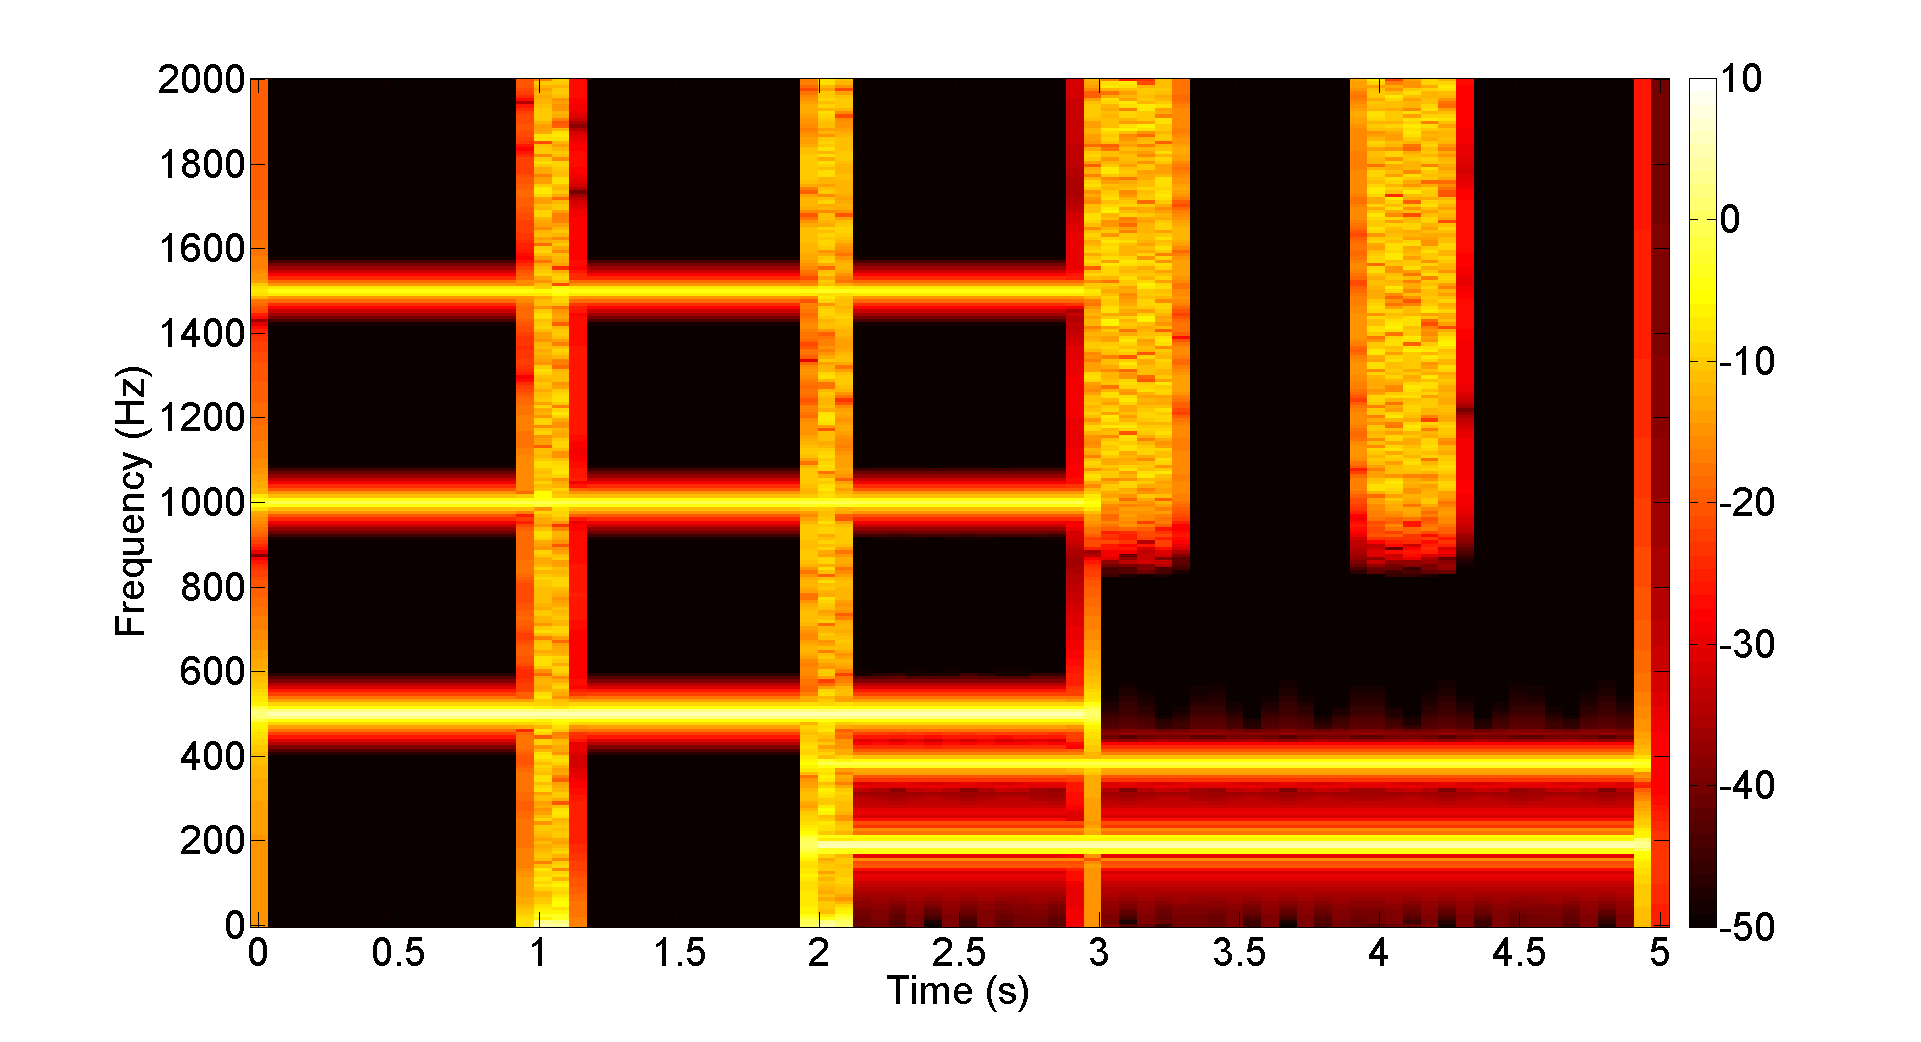
\includegraphics[width=9cm]{fig/synthetictestspectrogram.png}
%  \vspace{2.0cm}
  \caption{\label{SpectroSynth} Spectrogram of the synthetic test signals.}
  
\end{figure}

\begin{figure*}
   
	\centering    
  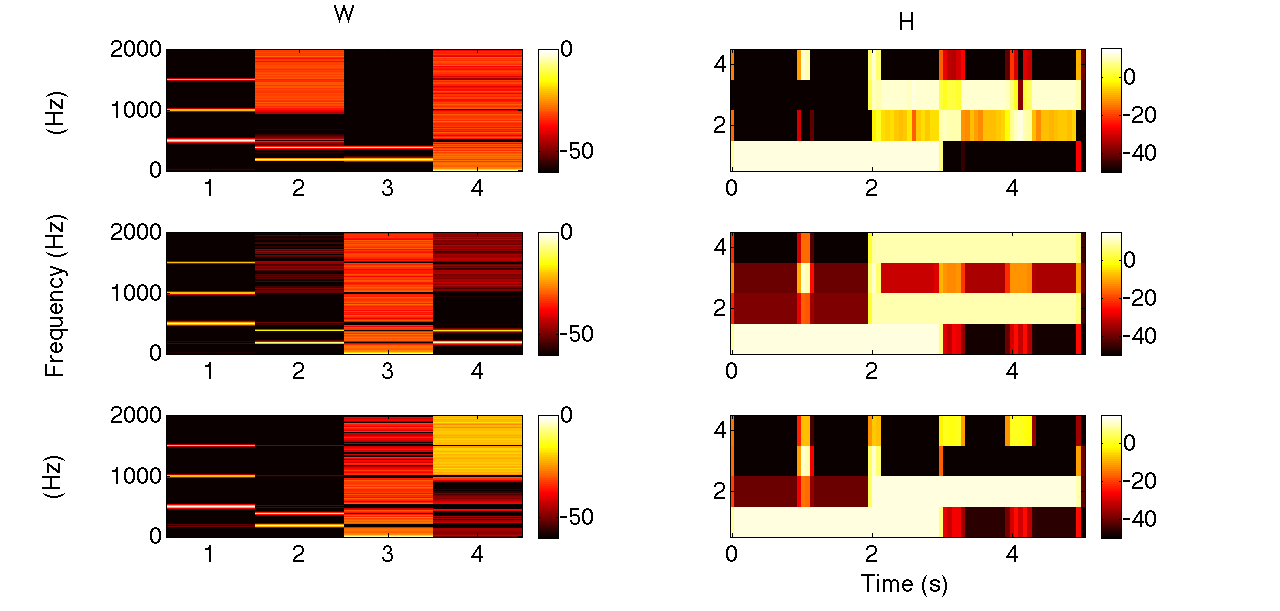
\includegraphics[width=15cm]{fig/WHcomp.png}

\caption{\label{resultONMF2} Results of the decomposition of the NMF (top matrices), PNMF (middle matrices) and SPNMF (bottom matrices).}


\end{figure*}


\subsection{Protocol and details of the test database}


To understand the behaviour of the SPNMF with the fixed dictionary (algorithm \ref{AlgoDictionary}), we run different tests on the public SiSec database from \cite{SiSec10}. It is composed of polyphonic real-world music excerpts. Each music signal contains percussive, harmonic instruments and vocals. It consists of four recordings of duration ranging from $14$ to $24$~s. The goal is to perform an harmonic/percussive decomposition. As in \cite{canadas2014percussive} we will not consider the vocal part and we will build mixture signals only from the percussive and harmonic instruments. All the signals are sampled at $44.1kHz$. We compute the STFT with a $1024$ and $2048$ sample-long Hann window with a $50\%$ overlap.
Three tests are run on these data. The first test aims at assessing the robustness of the SPNMF with respect to the rank of the PNMF part. The second test is to evaluate which of the three divergences (Euc, KL and IS respectively) give the best harmonic/percussive decomposition. The last test shows the influence of the dictionary on the separation performance. We are using a different database to set-up the proposed method from the one in the evaluation phase to prevent any possible training in order to make the comparison as fair as possible. 
In order to evaluate and compare the results we compute the common metric for blind source separation with the toolbox BSS-Eval \cite{bsseval}. 


\subsection{Robustness wrt the rank of the harmonic part}\label{setup:rank}

In the case where we use a dictionary matrix, the only parameter of the algorithm is the rank of factorization of the harmonic part. We used the SPNMF algorithm with the fixed dictionary obtained from the STFT of a drum signal as described in sec \ref{fixedict}. The algorithms are implemented using the multiplicative update rules from \ref{euclidisteq}, \ref{KLdisteq} and \ref{ISdisteq} and they are all initialized with the same random non-negative matrices. 
We display the mean value of the separation results on Figure \ref{RankOfFact}. When the rank of factorization is small, the Euclidean distance and the KL divergence do not obtain satisfying results however, for $r>=100$, the results for both distance are stable. With the IS divergence, the results are independent of the size of the factorization.

The optimization process of SPNMF is straight forward thanks to the robustness of the method to the value of the rank of factorization. The number of components that can be decomposed by orthogonal basis functions are limited and increasing the rank of factorization does not perturb the results as the harmonic part has to be orthogonal. For the rest of the article, the rank of factorization will be set to $r=100$ for all methods.



\begin{figure}[htb]

  \centering 
  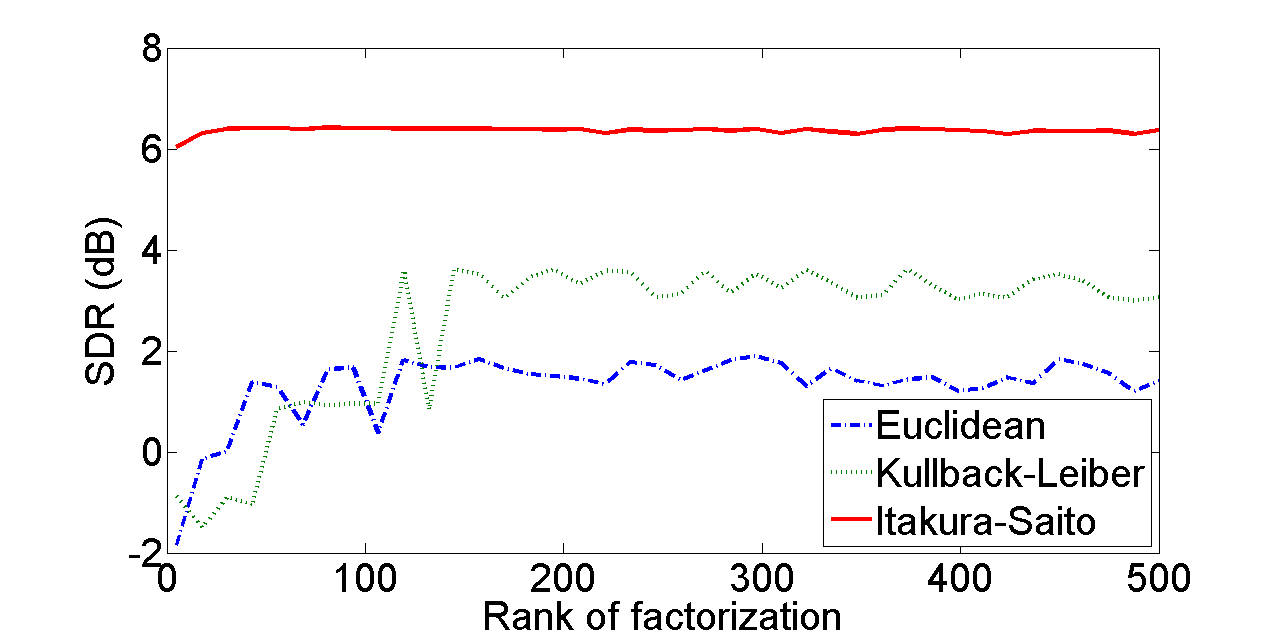
\includegraphics[width=9cm]{fig/RankOfFact.png}
%  \vspace{2.0cm}
  \caption{\label{RankOfFact} Optimization of the rank of factorization with the three divergences.}
  
\end{figure}




\subsection{Influence of the divergence}\label{setup:divergence}

In this section we discuss the influence of the divergence in the results of the SPNMF algorithm. It has been established that the IS divergence is well suited to audio signal decomposition \cite{gray1980distortion}, even if it does not always lead to superior separation performance \cite{canadas2014percussive}. In this section, we perform a test of the three divergences on the SiSec database to evaluate the performance of the three algorithms. We tried two different windows length ($1024$ samples and $2048$ samples) for the Fourier transform as it showed interesting results. We display on Figure \ref{frame1024} and \ref{frame2048} the mean of the results of the three algorithms on the SiSec database. Each box-plot is made up of a central line indicating the median of the data, upper and lower box edges indicating the $1^{st}$ and $3^{rd}$ quartiles, and whiskers indicating the minimum and maximum values. 

When the frame length is small, the percussive instruments are well represented and the energy is localized. Using a longer window spreads the percussive energy while the tonal components are well separated in the TF domain.

When the frame size is small, Figure \ref{frame1024} shows that the percussive decomposition is better for the Euclidean distance and the KL divergences, however, the harmonic components are not well separated in the TF domain, the orthogonal part of SPNMF does not perform a good separation.  
In the case of a long window, the Figure \ref{frame2048} shows that the IS divergence performs better than the other divergences. The orthogonal part is more effective to extract the harmonic components as the finer frequency resolution allows for a better separation in the TF domain. The scale invariant property of the IS divergence meaning that low energy components of the spectrogram bear the same relative importance as high energy ones, allows a good extraction of the percussive instruments even if the energy is spread temporally.


For the rest of the article, we will use the SPNMF algorithm with the IS divergence and a $2048$ window size in the STFT.


\begin{figure}[htb]

  \centering 
  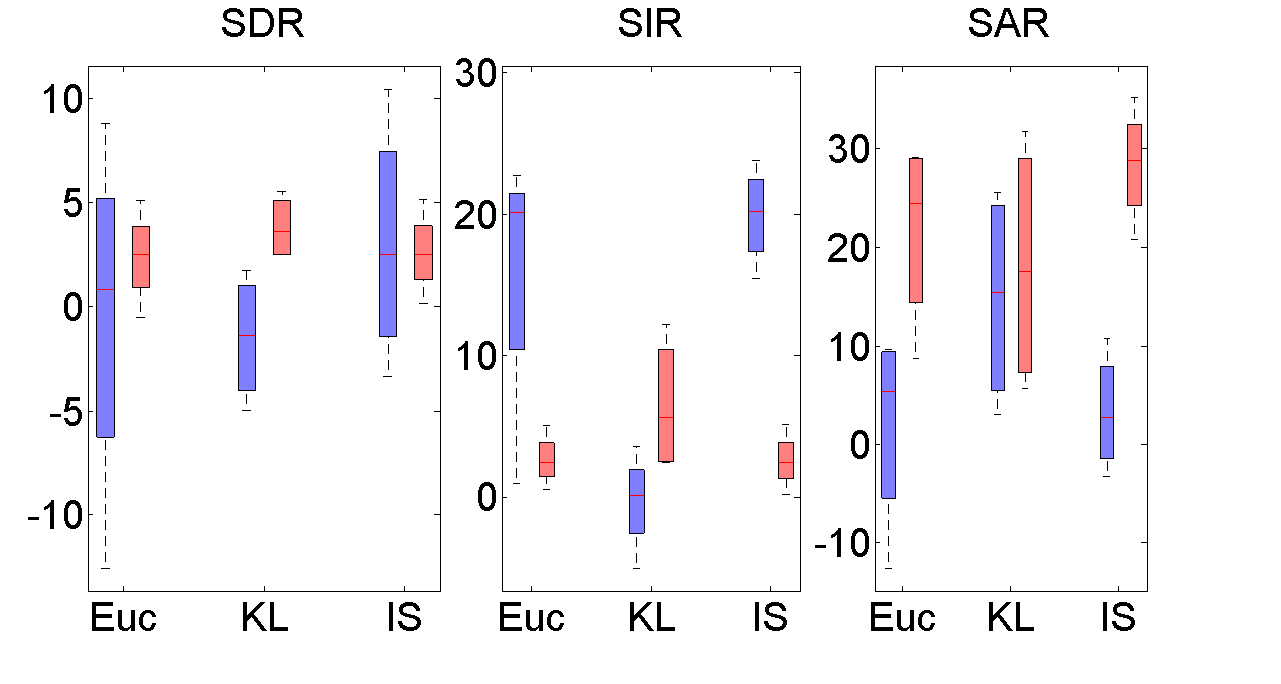
\includegraphics[width=9cm]{fig/DivergenceFrame1024.png}
%  \vspace{2.0cm}
  \caption{\label{frame1024} SDR, SIR and SAR of harmonic (left bar)/percussive (right bar) estimated sources on the SiSec database with a window frame of $1024$ samples.}
  
\end{figure}


\begin{figure}[htb]

  \centering 
  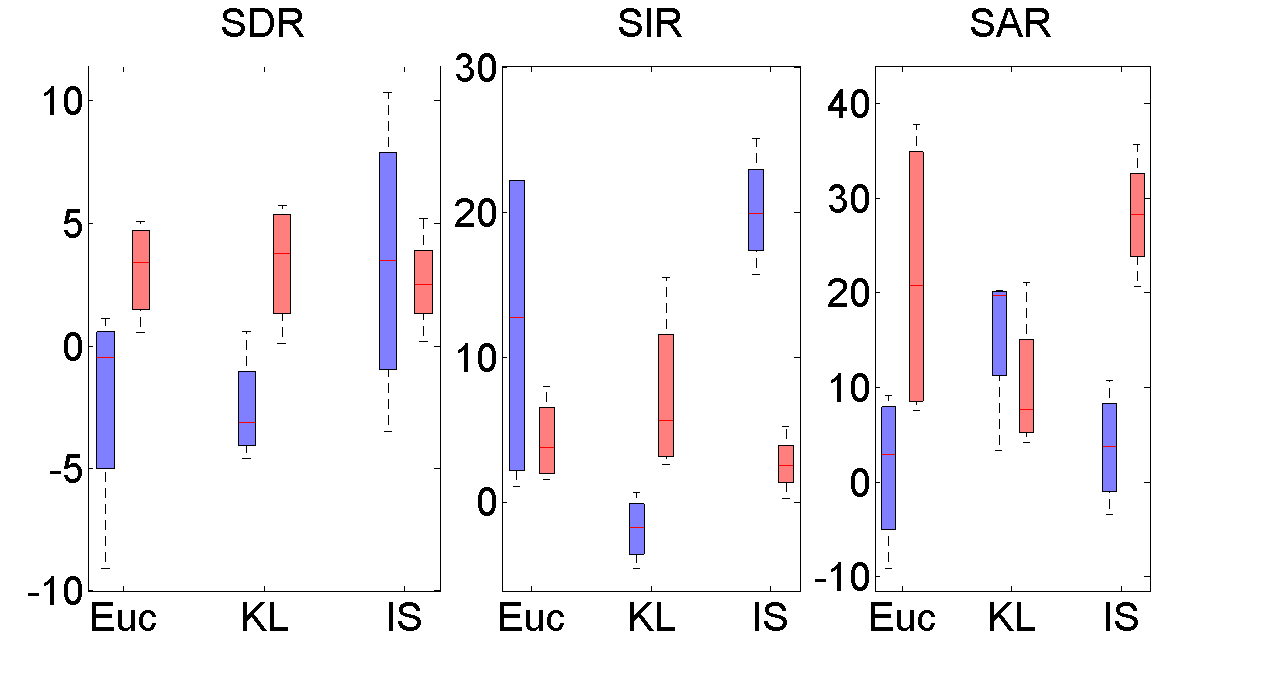
\includegraphics[width=9cm]{fig/DivergenceFrame2048.png}
%  \vspace{2.0cm}
  \caption{\label{frame2048} SDR, SIR and SAR of harmonic (left bar)/percussive (right bar) estimated sources on the SiSec database with a window frame of $2048$ samples.}
  
\end{figure}



\subsection{Influence of the dictionary}\label{setup:dictionary}

We now discuss the influence of the dictionary. We tried the two methods described in section \ref{fixedict} and a third dictionary is made by the concatenation of the two dictionaries. The more information contained is the dictionary, the more chance for the decomposition to properly extract the percussive part. On some signals the decomposition is not able to extract a lot of energy from the mixture as no atoms from the dictionary correspond to an atom of the percussive signal.
We display on the Figure \ref{resultsDict} the SDR results of the decomposition using the NMF dictionary, the STFT dictionary and the concatenated dictionary. The SAR and SIR are in the annexe at \ref{resultsDictSAR} and \ref{resultsDictSIR} respectively. On our tests, the results with the concatenated dictionary have the highest score. Indeed the concatenated dictionary contains the largest amount of information and as a result, obtains the best separation. As the dictionary is fixed it is important to have a large dictionary to extract a large type of percussive instruments. For the tests we will conduct later in Section \ref{sec:stateoftheart} on a large database, we will use the concatenated dictionary as it contains the largest amount of information. 


\begin{figure}[htb]

  \centering 
  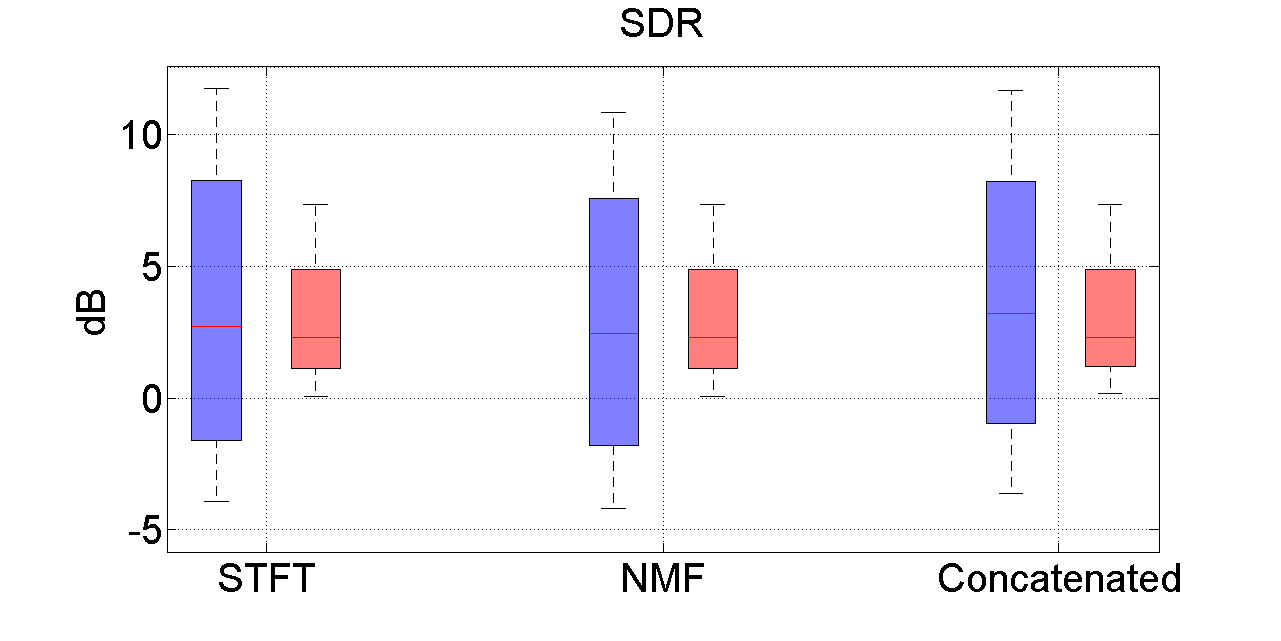
\includegraphics[width=8cm]{fig/DictSDR.png}
%  \vspace{2.0cm}
  \caption{\label{resultsDict} SDR of harmonic (left bar)/percussive (right bar) estimated sources on the SiSec database with a STFT dictionary, a NMF dictionary and the concatenation of the two.}
  
\end{figure}


%\begin{table}
%   
%	\centering    
%   \begin{tabular}{|l|l|l|l|l|}
%  \hline
%  &    & Percussive separation & Harmonic separation  \\
%  \hline
%       & NMF          & 10.28 & 2.69  \\
%  SDR  & STFT         & 10.17 & 2.59  \\
%  (dB) & Concatenated & 10.21 & 2.51  \\  
%  \hline
%       & NMF           & 20.97 & 2.45  \\
%  SIR  & STFT          & 21.11 & 2.61  \\
%  (dB) & Concatenated  & 20.70 & 2.65  \\  
%   \hline
%       & NMF           & 10.70 & 29.41  \\
%  SAR  & STFT          & 10.58 & 29.59  \\
%  (dB) & Concatenated  & 10.65 & 29.58  \\ 
%  \hline
%\end{tabular} 
%\caption{\label{resultsDict} Source separation performance using three dictionaries.}
%
%
%\end{table}
%\vspace{-0.4cm}
%



\section{State of the art Benchmark}\label{sec:stateoftheart}

In this section, we compare the proposed method with three state of the art methods on a large evaluation database. We detail first the database used and the other state of the art method in sec \ref{database} and \ref{soth} respectively.  


\subsection{Database}\label{database}

The dataset is taken from medley-dB \cite{bittner2014medleydb}, it is composed of polyphonic real-world music excerpts. It has $122$ music signals and $84$ of them contain percussive instruments, harmonic instruments and vocals. The signals that do not contain a percussive part are not part of the evaluation. The goal is to perform an harmonic/percussive decomposition as in \cite{canadas2014percussive} thus the vocal part is omitted. All the signals are sampled at $44.1kHz$.

\subsection{Other state of the art methods}\label{soth}

We compare here the SPNMF with the dictionary matrix with other recent state of the art methods: constrained NMF \cite{canadas2014percussive}, HPSS \cite{fitzgerald2010harmonic} and NMPCF \cite{kim2011nonnegative}. Constrained NMF and NMPCF are re-implemented in this paper and the HPSS implementation is taken from \cite{DriedgerMueller14_TSMToolbox_DAFX}.

HPSS is a state of the art, versatile and computationally efficient method. It is widely used in the Music Information Retrieval community and is a good baseline for comparison. The constrained NMF algorithm is the most recent method of harmonic/percussive separation. It gives good results on a small scale test, however the robustness of the algorithm has not been tested yet in a large scale experiment. Finally the NMPCF, similarly to our method, uses a drum dictionary to guide the percussive estimation but the harmonic part is totally unconstrained. 


\subsection{Results} \label{subResults}

Figures \ref{DatabaseSDR}, \ref{DatabaseSIR} and \ref{DatabaseSAR} show the SDR, SIR and SAR results of the four methods on the selected $84$ songs of the original Medley-dB database \cite{bittner2014medleydb}. The results on the entire database show that the four methods extract the harmonic instruments much better than the percussive instruments. All methods rely on Weiner filtering for phase reconstruction (see equation \ref{percuweiner}). As the percussive instruments have flat spectra, the percussive mask is a non sparse matrix and small estimation errors drastically decrease the results of the percussive instruments. This tendency is not visible on small scale tests as it is not always the case (see table \ref{resultsDict}). 
Figure \ref{DatabaseSDR} shows that SPNMF obtains on average the highest separation score for the percussive, harmonic and mean SDR. However, the variance of the results of SPNMF is higher than for the other algorithms. Some songs of the database contain percussive instruments that are not present in the learning database ENST-Drums, for example tambourine, bongo, gong and electronic drums. Because the dictionary is fixed, the percussive instruments are not correctly decomposed by the SPNMF. It induces an increase of the variance as some songs are well separated while other obtain much lower results as the percussive part is not well decomposed.

The NMPCF, also based on trained data, is more robust than SPNMF because the dictionary that extract the drums is not fixed. It allows more freedom and the results are more consistent even if some percussive instruments are not in the learning database. However, the mean score is lower than the SPNMF.

The HPSS results obtained in our tests are unsatisfying. A wide variety of harmonic instruments in the database have really strong transients and rich harmonic spectra (distorted electric guitar, glockenspiel,...), similarly, some percussive instruments have sparse basis functions localised in the low frequency range (bass drum, bongo, toms,...). Because of that, HPSS fails to extract these instruments in the appropriate harmonic/percussive parts. On average, it is able to correctly separate the percussive part (with relatively high SDR and the highest SIR) but with a very low SAR compared to the other methods. \cite{canadas2014percussive} observed similar outcomes for HPSS.

Similarly, the constrained NMF algorithm relies on the same hypothesis as HPSS and the results are lower than those of SPNMF. Some transients of the harmonic instruments are decomposed in the percussive part, and some percussive instruments (mainly in the low frequency range) are decomposed by the harmonic part. The method is still competitive in the large scale test. 

Compared to the other state of the art methods, SPNMF obtains the higher average results on the selected database. 


\begin{figure}[h]

  \centering 
  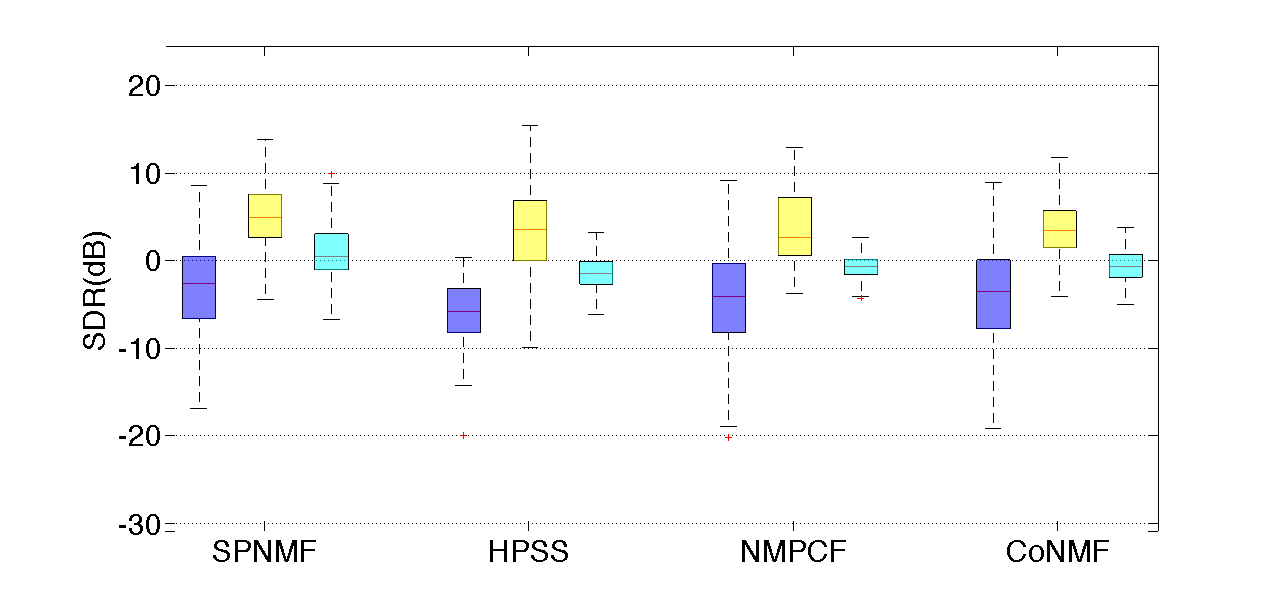
\includegraphics[width=9cm]{fig/DatabaseSDR.png}
%  \vspace{2.0cm}
  \caption{\label{DatabaseSDR} SDR for percussive/left, harmonic/middle, mean/right separation results on the database for the four methods.}
  
\end{figure}

\begin{figure}[h]

  \centering 
  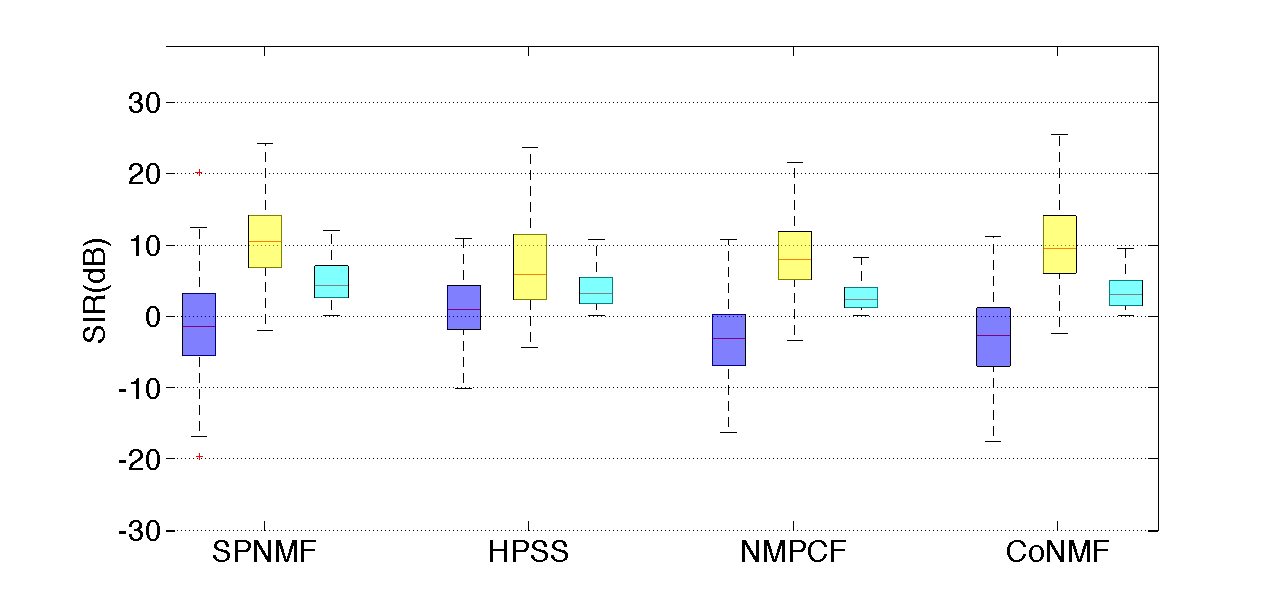
\includegraphics[width=9cm]{fig/DatabaseSIR.png}
%  \vspace{2.0cm}
  \caption{\label{DatabaseSIR} SIR for percussive/left, harmonic/middle, mean/right separation results on the database for the four methods.}
  
\end{figure}

\begin{figure}[h]

  \centering 
  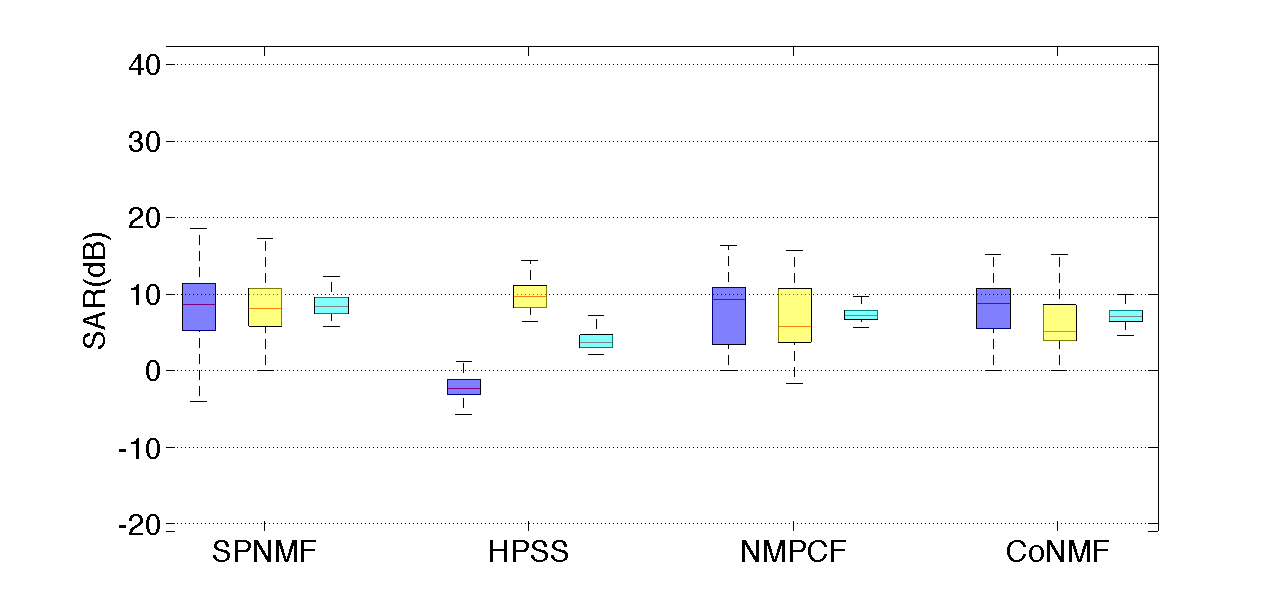
\includegraphics[width=9cm]{fig/DatabaseSAR.png}
%  \vspace{2.0cm}
  \caption{\label{DatabaseSAR} SAR for percussive/left, harmonic/middle, mean/right separation results on the database for the four methods.}
  
\end{figure}




\subsection{Results on a genre specific database}\label{sec:subdata}

The individual results on most of the songs of the database are similar to the average results. However, some interesting results were found on specific genre of music. Here we present the results obtained on $14$ songs of "Electronic/Fusion". These songs for the most part have a lot of silence and some solo parts where only one instrument is playing. Finally on some songs, the electronic drum reproduces the same pattern for the whole song so the drum part is very redundant.

Figure \ref{ElectroFusionSDR} shows the SDR results of the four methods on the sub-database. The SIR and SAR results are in the annexe as Figure \ref{ElectroFusionSIR} and \ref{ElectroFusionSAR} respectively. 


The HPSS method gives competitive results, with a low variance for the percussive results and good overall mean. The HPSS obtains consistent results throughout the database. The results on the genre specific database are significantly better than on the whole database. It traduces the fact that the harmonic/percussive instruments are easier to separate on these songs. 
 
The results of NMPCF are the lowest of the four methods. The Unconstrained harmonic part gives the NMPCF a higher degree of freedom that decreases the score as the information is unequally distributed in the harmonic and percussive layer depending on the signal to decompose. 

Finally constrained NMF does not obtain satisfying results on this sub-database. The hyper-parameters are set to the optimal values obtained on a training database of another genre. Because of that, the value of the parameters are not set correctly and similarly to NMPCF, the information is not distributed in the appropriate harmonic/percussive parts. 


On this sub-database, SPNMF outperforms considerably the other methods. Similarly to section \ref{subResults}, the percussive decomposition of SPNMF has high variance because some of the instruments are not in the learning database. However, the mean of the percussive decomposition is significantly higher than constrained NMF and NMPCF also the harmonic decomposition and the mean results of SPNMF are clearly above all the other methods. SPNMF is effective to extract the redundant drum parts. Also as the drum dictionary is fixed, it is unlikely for the percussive part to extract harmonic components, similarly, as the columns of $W$ are orthogonal, it is unlikely for the harmonic part to extract percussive components. Contrary to other algorithms, when the harmonic or percussive instruments are playing alone, the SPNMF does not extract any information in the percussive or harmonic part respectively.



\begin{figure}[htb]

  \centering 
  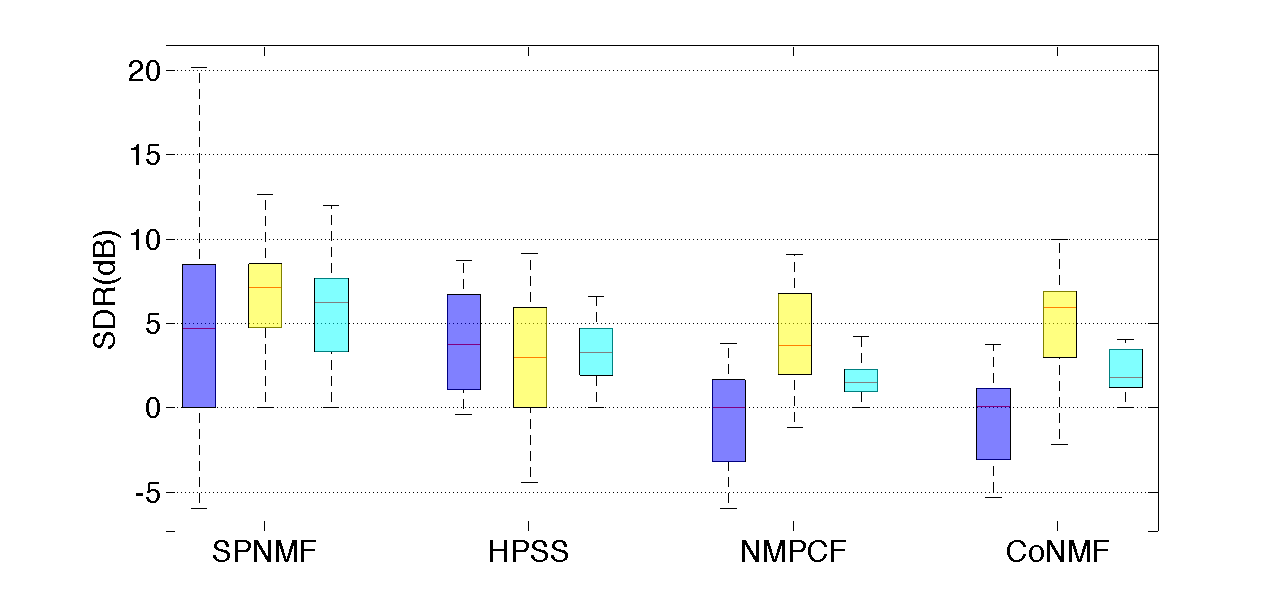
\includegraphics[width=9cm]{fig/ElectroFusionSDR.png}
%  \vspace{2.0cm}
  \caption{\label{ElectroFusionSDR} SDR for percussive/left, harmonic/middle, mean/right separation results on the Electronic/Fusion songs for the four methods.}
  
\end{figure}

\subsection{Discussion}\label{discu}

The results on the entire database give us insightful information.
HPSS and constrained NMF use the hypothesis that harmonic instruments have sparse tonal spectrogram and percussive instruments have flat transient spectra. They utilize two different methods to extract the instruments (complementary median filtering, and constraints on the NMF decomposition).
NMPCF uses prior learning to extract the percussive instruments in a specific part while the harmonic instruments are decomposed in an unconstrained layer. 
Finally, SPNMF uses both techniques from the previous state of the art methods. It utilities prior learning to extract the percussive instruments while the harmonic parts are extracted by the sparse PNMF components.



Each methods have their advantages and their drawbacks. HPSS is the easiest method to implement, the fastest and it does not require any hyper-parameter tuning. The results of HPSS can be competitive when the harmonic instruments have smooth transients (i.e., sustained instruments as flute, violin) and the percussive instruments have flat spectra (i.e., cymbal, snare drum). However, when the harmonic instruments have strong transients (glockenspiel, piano) and the percussive instruments have sparse spectra (bass drum, bongo) the HPSS does not obtain good results. 

The constrained NMF is based on the same hypothesis than HPSS and has the same problem. Fine tuning of the hyper-parameters can alleviate the problem mentioned above but it is a tedious process and is not possible in the case of blind source separation. Our tests on a large database show that the constrained NMF is not robust to a wide variability of the analyzed signals.

Contrary to the results from \cite{canadas2014percussive} the NMPCF algorithm gives competitive results compare to HPSS and constrained NMF. As it uses training to guide the decomposition process, it requires a wide variety of information to perform on a large scale test. If the training database does not contain sufficient information, the results will not be satisfying. 

On the large scale test, SPNMF outperforms the other methods. It is able to extract the harmonic and the percussive instruments with higher score for SDR, SAR and SIR. Using prior dictionary learning with a physical model on the harmonic instruments help to separate the instruments with much better accuracy.

In our test, the training database of SPNMF and NMPCF is only composed of drum sounds, however the database \cite{bittner2014medleydb} contains a wide variety of percussive instruments that are not in the training database. We decided not to include these types of percussion in the training database as we wanted to have a comparable computation time between the four methods and to test the robustness of the supervised methods when a percussive signal is not in the database. 


\section{Conclusion}
\label{sec:conc}

In this article, we demonstrate that SPNMF is a very promising model for harmonic/percussive decomposition. Indeed, the SPNMF outperforms the other state of the methods on the medley-dB database \cite{bittner2014medleydb}. Carrying out an evaluation on a large database allowed us to judge more accurately the performance of the four methods on a large variety of music signals. We can also say that the information from the drum dictionary built from the database ENST-Drums \cite{gillet2006enst} is not sufficient to perform an harmonic/percussive source separation on a large scale. Depending of the style of music, some drums share similarities. A possible improvement would be to build genre specific drum dictionaries. This way the computation time is reasonable as the amount information could be reduced as the templates of the dictionary could be a lot more focused on specific type of drums. 


On a large database none of the state of the art methods produce a satisfying harmonic/percussive source separation. The large variety of audio signal makes the task extremely difficult. However, on a smaller section of the database, the SPNMF showed some promising results (see \ref{sec:subdata}).





\section*{Annexe}

\subsection{Euclidean distance}\label{euclidisteq}
The euclidean distance gives us the problem,
$$\min_{W_1,W_2,H_2 \geq 0} \|V - W_{1}W_{1}^{T}V + W_{2} H_{2} \|^2.$$
The gradient wrt $W_1$ gives the update
$$[\nabla_{W_1} D(V|\tilde{V})]^{-} = 2 VV^TW_1, $$
and
\begin{align*}
[\nabla_{W_1} D(V|\tilde{V})]^{+} = 2VH_2^TW_2^TW_1 + W_2H_2V^TW_1 + \\ VV^TW_1W_1^TW_1 + W_1W_1^TVV^TW_1.
\end{align*}

Similarly, the gradient wrt $W_2$ gives
$$ [\nabla_{W_2} D(V|\tilde{V})]^{-} = VH_2^T $$
and
$$ [\nabla_{W_2} D(V|\tilde{V})]^{+} = 2W_1W_1^TVH_2^T + W_2H_2H_2^T.$$

Finally, the gradient wrt $H_2$ gives
$$ [\nabla_{H_2} D(V|\tilde{V})]^{-} = W_2^TV  $$
and
$$ [\nabla_{H_2} D(V|\tilde{V})]^{+} = 2W_2^TW_1W_1^TV + W_2^TW_2H_2. $$


\subsection{Kullback Leiber divergence}\label{KLdisteq}
The Kullback Leiber divergence gives us the problem,
$$\min_{W_1,W_2,H_2 \geq 0} V(log(V) - log(\tilde{V})) + (V-\tilde{V}).$$

The gradient wrt $W_1$ gives
$$[\nabla_{W_1} D(V|\tilde{V})]_{i,j}^{-} = (ZV^TW_1)_{i,j} + (VZ^TW_1)_{i,j},$$
with $Z_{i,j} = (\frac{V}{W_1W_1^TV + W_2H_2})_{i,j}$. The positive part of the gradient is
$$[\nabla_{W_1} D(V|\tilde{V})]^{+}_{i,j} = \sum_k(W^TV)_{j,k} + (\sum_{k}V_{i,k})(\sum_a W_{a,j}).$$


Similarly, the gradient wrt $W_2$ gives
$$ [\nabla_{W_2} D(V|\tilde{V})]^{-} = VH_2^T $$
and
$$ [\nabla_{W_2} D(V|\tilde{V})]^{+} = W_1W_1^TVH_2^T + W_2H_2H_2^T.$$

Finally, the gradient wrt $H_2$ gives
$$ [\nabla_{H_2} D(V|\tilde{V})]^{-} = W_2^TV  $$
and
$$ [\nabla_{H_2} D(V|\tilde{V})]^{+} = 2W_2^TW_1W_1^TV + W_2^TW_2H_2. $$

 
\subsection{Itakura Saito divergence}\label{ISdisteq}
The Itakura Saito divergence gives us the problem,
$$\min_{W_1,W_2,H_2 \geq 0} \frac{V}{\tilde{V}} - log(\frac{V}{\tilde{V}}) +1.$$

The gradient wrt $W_1$ gives
$$[\nabla_{W_1} D(V|\tilde{V})]_{i,j}^{-} = (ZV^TW_1)_{i,j} + (VZ^TW_1)_{i,j},$$
with $Z_{i,j} = (\frac{V}{W_1W_1^TV + W_2H_2})_{i,j}$. 
The positive part of the gradient is
$$[\nabla_{W_1} D(V|\tilde{V})]_{i,j}^{-} = (\phi V^TW_1)_{i,j} + (V \phi^T W_1)_{i,j},$$
with $$ \phi_{i,j} = (\frac{I}{W_1W_1^TV + W_2H_2})_{i,j}.$$ and $I = ones(size(V))$.


Similarly, the gradient wrt $W_2$ gives
$$ [\nabla_{W_2} D(V|\tilde{V})]^{-} = VH_2^T $$
and
$$ [\nabla_{W_2} D(V|\tilde{V})]^{+} = W_1W_1^TVH_2^T + W_2H_2H_2^T.$$

Finally, the gradient wrt $H_2$ gives
$$ [\nabla_{H_2} D(V|\tilde{V})]^{-} = W_2^TV  $$
and
$$ [\nabla_{H_2} D(V|\tilde{V})]^{+} = 2W_2^TW_1W_1^TV + W_2^TW_2H_2. $$



\subsection{SAR and SIR results with the different dictionaries}

\begin{figure}[htb]

  \centering 
  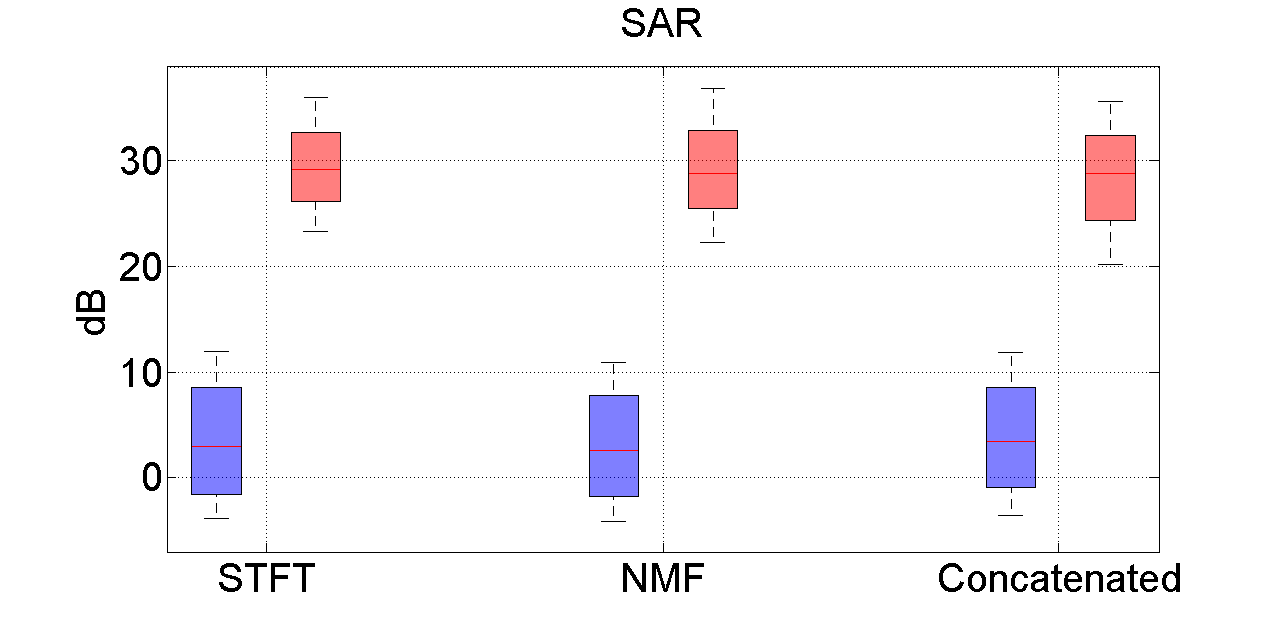
\includegraphics[width=8cm]{fig/DictSAR.png}
%  \vspace{2.0cm}
  \caption{\label{resultsDictSAR} SAR of harmonic (left bar)/percussive (right bar) estimated sources on the SiSec database with a STFT dictionary, a NMF dictionary and the concatenation of the two.}
  
\end{figure}
\begin{figure}[htb]

  \centering 
  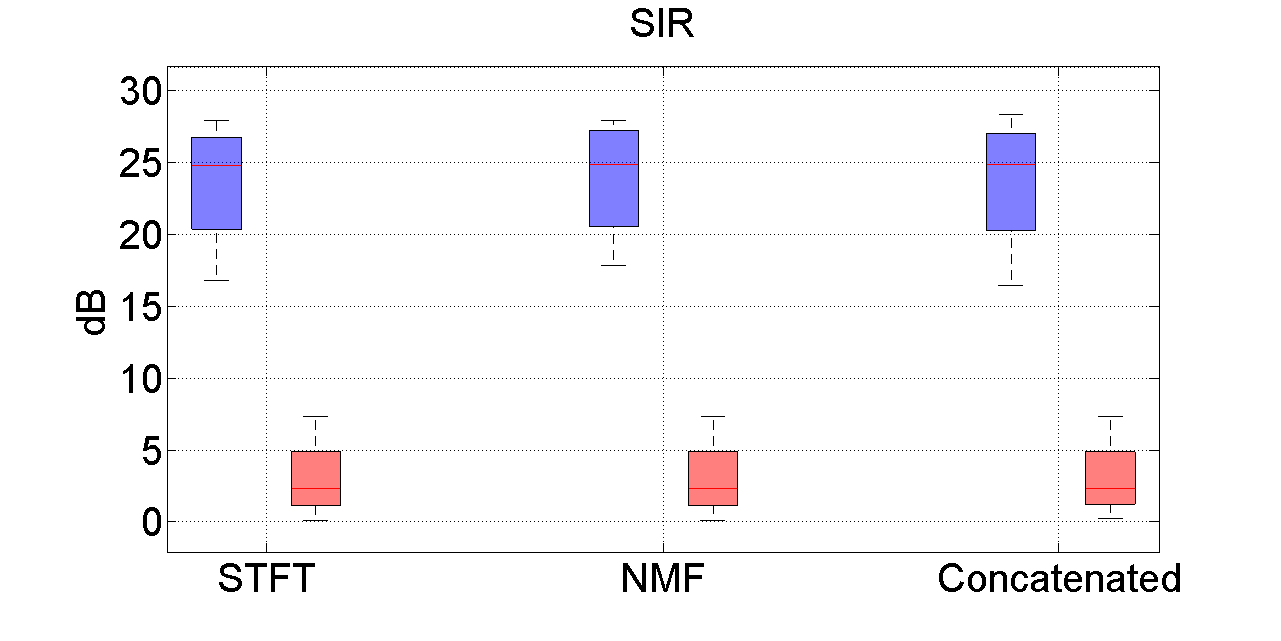
\includegraphics[width=8cm]{fig/DictSIR.png}
%  \vspace{2.0cm}
  \caption{\label{resultsDictSIR} SIR of harmonic (left bar)/percussive (right bar) estimated sources on the SiSec database with a STFT dictionary, a NMF dictionary and the concatenation of the two.}
  
\end{figure}

\subsection{Results on the sub database}

\begin{figure}[h]

  \centering 
  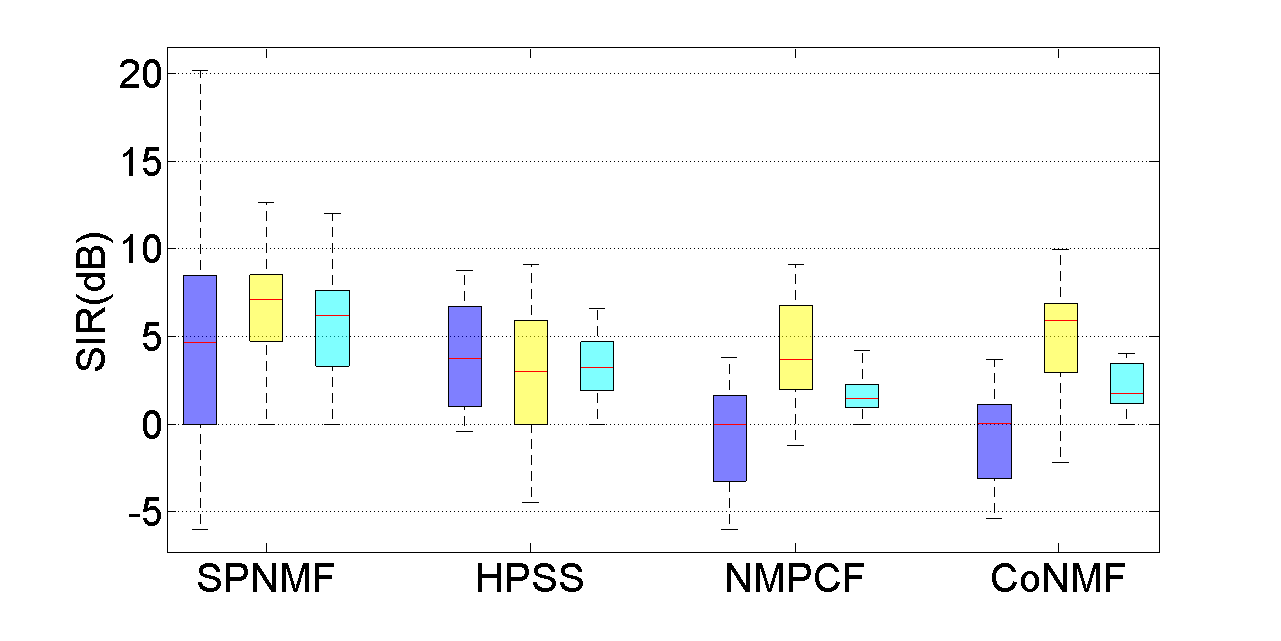
\includegraphics[width=9cm]{fig/ElectroFusionSIR.png}
%  \vspace{2.0cm}
  \caption{\label{ElectroFusionSIR} SIR for percussive/left, harmonic/middle, mean/right separation results on the Electronic/Fusion songs for the four methods.}
  
\end{figure}

\begin{figure}[h]

  \centering 
  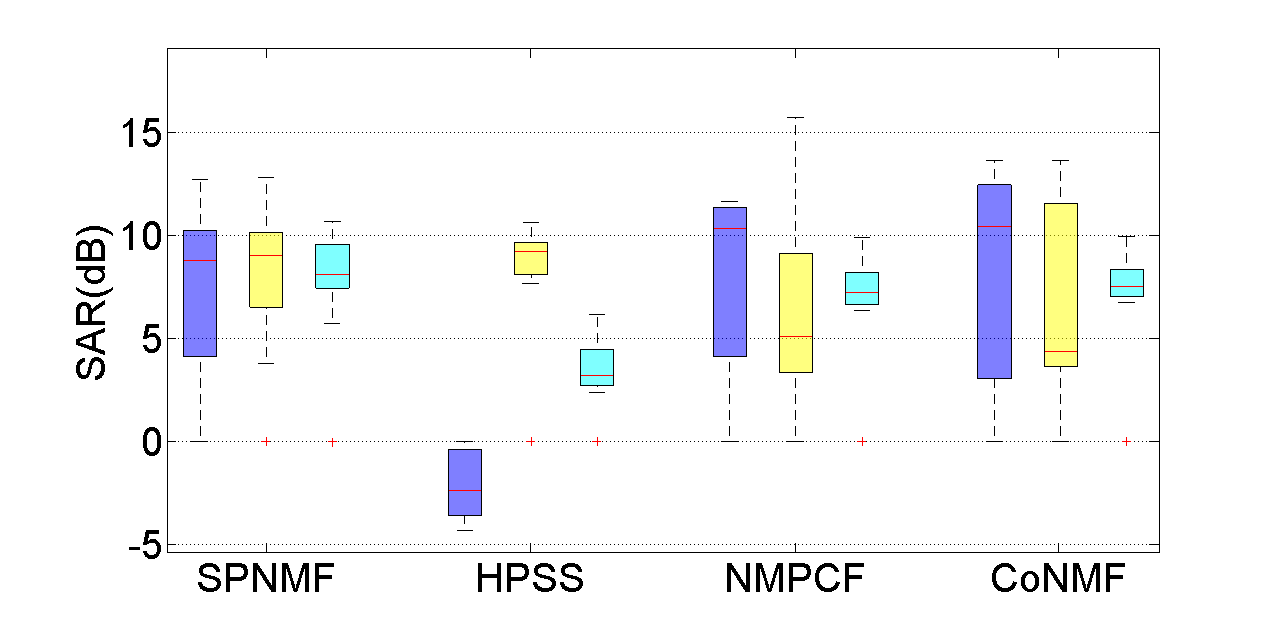
\includegraphics[width=9cm]{fig/ElectroFusionSAR.png}
%  \vspace{2.0cm}
  \caption{\label{ElectroFusionSAR} SAR for percussive/left, harmonic/middle, mean/right separation results on the Electronic/Fusion songs for the four methods.}
  
\end{figure}


\section*{Acknowledgment}


The authors would like to thank...


% Can use something like this to put references on a page
% by themselves when using endfloat and the captionsoff option.
\ifCLASSOPTIONcaptionsoff
  \newpage
\fi



% trigger a \newpage just before the given reference
% number - used to balance the columns on the last page
% adjust value as needed - may need to be readjusted if
% the document is modified later
%\IEEEtriggeratref{8}
% The "triggered" command can be changed if desired:
%\IEEEtriggercmd{\enlargethispage{-5in}}

% references section

% can use a bibliography generated by BibTeX as a .bbl file
% BibTeX documentation can be easily obtained at:
% http://www.ctan.org/tex-archive/biblio/bibtex/contrib/doc/
% The IEEEtran BibTeX style support page is at:
% http://www.michaelshell.org/tex/ieeetran/bibtex/
\bibliographystyle{IEEEtran}
% argument is your BibTeX string definitions and bibliography database(s)
\bibliography{reference}
%
% <OR> manually copy in the resultant .bbl file
% set second argument of \begin to the number of references
% (used to reserve space for the reference number labels box)
%\begin{thebibliography}{1}
%
%\bibitem{IEEEhowto:kopka}
%H.~Kopka and P.~W. Daly, \emph{A Guide to \LaTeX}, 3rd~ed.\hskip 1em plus
%  0.5em minus 0.4em\relax Harlow, England: Addison-Wesley, 1999.
%
%\end{thebibliography}
%
% biography section
% 
% If you have an EPS/PDF photo (graphicx package needed) extra braces are
% needed around the contents of the optional argument to biography to prevent
% the LaTeX parser from getting confused when it sees the complicated
% \includegraphics command within an optional argument. (You could create
% your own custom macro containing the \includegraphics command to make things
% simpler here.)
%\begin{IEEEbiography}[{\includegraphics[width=1in,height=1.25in,clip,keepaspectratio]{mshell}}]{Michael Shell}
% or if you just want to reserve a space for a photo:

\begin{IEEEbiography}{Michael Shell}
Biography text here.
\end{IEEEbiography}

% if you will not have a photo at all:
\begin{IEEEbiographynophoto}{John Doe}
Biography text here.
\end{IEEEbiographynophoto}

% insert where needed to balance the two columns on the last page with
% biographies
%\newpage

\begin{IEEEbiographynophoto}{Jane Doe}
Biography text here.
\end{IEEEbiographynophoto}

% You can push biographies down or up by placing
% a \vfill before or after them. The appropriate
% use of \vfill depends on what kind of text is
% on the last page and whether or not the columns
% are being equalized.

%\vfill

% Can be used to pull up biographies so that the bottom of the last one
% is flush with the other column.
%\enlargethispage{-5in}



% that's all folks
\end{document}


